\documentclass[a4paper]{article}
\usepackage[ngerman]{babel}
\usepackage[utf8]{inputenc}
\usepackage{multicol}
\usepackage{calc}
\usepackage{ifthen}
\usepackage[landscape]{geometry}
\usepackage{amsmath,amsthm,amsfonts,amssymb}
\usepackage{color,graphicx,overpic}
\usepackage{xcolor, listings}
\usepackage[compact]{titlesec} %less space for headers
\usepackage{mdwlist} %less space for lists
\usepackage{pdflscape}
\usepackage{verbatim}
\usepackage[most]{tcolorbox}
\usepackage[hidelinks,pdfencoding=auto]{hyperref}
\usepackage{bussproofs}
\usepackage{fancyhdr}
\usepackage{lastpage}
\pagestyle{fancy}
\fancyhf{}
\fancyhead[L]{Grundlagen der Biosignalverarbeitung}
\fancyfoot[L]{\thepage/\pageref{LastPage}}
\renewcommand{\headrulewidth}{0pt} %obere Trennlinie
\renewcommand{\footrulewidth}{0pt} %untere Trennlinie

\pdfinfo{
 /Title (Grundlagen der Biosignalverarbeitung - Cheatsheet)
 /Creator (TeX)
 /Producer (pdfTeX 1.40.0)
 /Author (Robert Jeutter)
 /Subject ()
}

%%% Code Listings
\definecolor{codegreen}{rgb}{0,0.6,0}
\definecolor{codegray}{rgb}{0.5,0.5,0.5}
\definecolor{codepurple}{rgb}{0.58,0,0.82}
\definecolor{backcolour}{rgb}{0.95,0.95,0.92}
\lstdefinestyle{mystyle}{
 backgroundcolor=\color{backcolour}, 
 commentstyle=\color{codegreen},
 keywordstyle=\color{magenta},
 numberstyle=\tiny\color{codegray},
 stringstyle=\color{codepurple},
 basicstyle=\ttfamily,
 breakatwhitespace=false, 
}
\lstset{style=mystyle, upquote=true}

%textmarker style from colorbox doc
\tcbset{textmarker/.style={%
 enhanced,
 parbox=false,boxrule=0mm,boxsep=0mm,arc=0mm,
 outer arc=0mm,left=2mm,right=2mm,top=3pt,bottom=3pt,
 toptitle=1mm,bottomtitle=1mm,oversize}}

% define new colorboxes
\newtcolorbox{hintBox}{textmarker,
 borderline west={6pt}{0pt}{yellow},
 colback=yellow!10!white}
\newtcolorbox{importantBox}{textmarker,
 borderline west={6pt}{0pt}{red},
 colback=red!10!white}
\newtcolorbox{noteBox}{textmarker,
 borderline west={3pt}{0pt}{green},
 colback=green!10!white}

% define commands for easy access
\renewcommand{\note}[2]{\begin{noteBox} \textbf{#1} #2 \end{noteBox}}
\newcommand{\warning}[1]{\begin{hintBox} \textbf{Warning:} #1 \end{hintBox}}
\newcommand{\important}[1]{\begin{importantBox} \textbf{Important:} #1 \end{importantBox}}


% This sets page margins to .5 inch if using letter paper, and to 1cm
% if using A4 paper. (This probably isn't strictly necessary.)
% If using another size paper, use default 1cm margins.
\ifthenelse{\lengthtest { \paperwidth = 11in}}
 { \geometry{top=.5in,left=.5in,right=.5in,bottom=.5in} }
 {\ifthenelse{ \lengthtest{ \paperwidth = 297mm}}
 {\geometry{top=1.3cm,left=1cm,right=1cm,bottom=1.2cm} }
 {\geometry{top=1.3cm,left=1cm,right=1cm,bottom=1.2cm} }
 }

% Redefine section commands to use less space
\makeatletter
\renewcommand{\section}{\@startsection{section}{1}{0mm}%
 {-1ex plus -.5ex minus -.2ex}%
 {0.5ex plus .2ex}%x
 {\normalfont\large\bfseries}}
\renewcommand{\subsection}{\@startsection{subsection}{2}{0mm}%
 {-1explus -.5ex minus -.2ex}%
 {0.5ex plus .2ex}%
 {\normalfont\normalsize\bfseries}}
\renewcommand{\subsubsection}{\@startsection{subsubsection}{3}{0mm}%
 {-1ex plus -.5ex minus -.2ex}%
 {1ex plus .2ex}%
 {\normalfont\small\bfseries}}
\makeatother

% Don't print section numbers
\setcounter{secnumdepth}{0}

\setlength{\parindent}{0pt}
\setlength{\parskip}{0pt plus 0.5ex} 
% compress space
\setlength\abovedisplayskip{0pt}
\setlength{\parskip}{0pt}
\setlength{\parsep}{0pt}
\setlength{\topskip}{0pt}
\setlength{\topsep}{0pt}
\setlength{\partopsep}{0pt}
\linespread{0.5}
\titlespacing{\section}{0pt}{*0}{*0}
\titlespacing{\subsection}{0pt}{*0}{*0}
\titlespacing{\subsubsection}{0pt}{*0}{*0}

\begin{document}

\raggedright
\begin{multicols}{3}\scriptsize
  % multicol parameters
  % These lengths are set only within the two main columns
  %\setlength{\columnseprule}{0.25pt}
  \setlength{\premulticols}{1pt}
  \setlength{\postmulticols}{1pt}
  \setlength{\multicolsep}{1pt}
  \setlength{\columnsep}{2pt}


  \section{Sensorik}

  Im Normalfall werden Sensoren verwendet, die eine physikalische oder
  chemische Größe in ein elektrisches Signal umwandeln bzw. eine
  elektrische Größe beeinflussen, die weiter verarbeitet werden können.
  Eine Umwandlung der Energieform der Biosignale ist notwendig. Selbst bei
  Sensoren für elektrische Größen ist eine Umwandlung (von Ionenleitung
  zur Elektronenleitung) nötig.

  Weitere Sensorengruppen, wie Temperatur-und chemische Sensoren werden
  hier nicht behandelt, da ihre Dynamik aus Sicht der BSA vernachlässigbar
  gering ist.


  \subsection{Klassifikation von Sensoren}

  Ein Sensor (lateinisch 'sensus': Gefühl) oder Fühler ist ein technisches
  Bauteil, das die physikalischen oder chemischen Eigenschaften (z.B.
  Wärmestrahlung, Temperatur, Feuchtigkeit, Druck, Schall, Helligkeit,
  Magnetismus, Beschleunigung, Kraft, elektrisches Potential) erfassen und
  in ein elektronisches oder ein anderes geeignetes Signal umwandeln kann.

  Man unterscheidet zwischen aktiven und passiven Sensoren

  \begin{itemize*}
    \item Aktiver Sensor: gibt eine Spannung oder einen Strom ab, wobei er für seine Funktion elektrische Energie benötigt oder eine Energieart in die elektrische umwandelt. Er wirkt wie eine elektrische Signalquelle (z.B. Phototransistor)
    \item Passiver Sensor: ändert elekttrische Größen (z.B. den Widerstand des Dehnmessstreifens in Abhängigkeit von der Dehnung) ohne Energiezufuhr von außen.
  \end{itemize*}

  Auflösung von Sensoren:

  \begin{itemize*}
    \item temporal: Zeitabstand zwischen Messungen (z.B. Geigerzähler, Aktionspotentiale)
    \item spektral: Abstand von Spektrallinien (z.B. Wärmebildkamera, Infrarotsensor, Spektralphotometer)
    \item räumlich: räumlicher Abstand (z.B. EEG, Ultraschall, CT/MRT)
    \item und alle Kombinationen (z.B. spatialtemporale Auflösung in einem Frequenzband)
  \end{itemize*}

  Klassifikation nach Messgröße:

  \begin{itemize*}
    \item Physikalisch: Kraft, Druck, Moment, Durchfluss
    \item Elektrizität: Potential, Strom, Impedanz
    \item Magnetismus: Fluss, Induktion
    \item Optik/Licht: spektrale Dämpfung, Extinktion
    \item Chemisch: Partialdruck von Gasen, Zucker, Hämoglobin
    \item Akustik: Herzschalltöne, Atmung
    \item Temperatur: Körpertemperatur
  \end{itemize*}

  \subsection{Druck, Dehnung und Kraft}

  Dehnmessstreifen (DMS)

  \begin{itemize*}
    \item Messprinzip: Dehnungsabhängiger Widerstand
    \item Realisierung: Widerstandsdraht oder Halbleiter als Gitter auf Träger
    \item Messbare Größen: Kraft, Druck, Moment
    \item Anwendung in der Medizintechnik: Atmungsdiagnostik, Fahrradergometer, Diagnostik des Bewegungsapparates
    \item Signaleigenschaftem
    \begin{itemize*}
      \item passiver Sensor - thermisches und/oder Halbleiter-Rauschen
      \item empfindlich gegen NF-elektrische/magnetische und HF-elektromagnetische Felder
      \item temperaturabhängig vor allem Halbleiter
      \item Übertragungseigenschaften abhängig von der Sensorkopplung
      \item Signaldynamik abhängig von Masse und Technologie  \end{itemize*}
  \end{itemize*}

  Grundlage ist der piezoresestive Widerstandseffekt: Durch Zug/Druck
  nimmt der elektrische Widerstand zu/ab

  \begin{itemize*}
    \item \$R=\textbackslash ro\textbackslash frac\{l\}\{A\}=\textbackslash ro\textbackslash frac\{4l\}\{d\^{}2\textbackslash pi\}\$, \$\textbackslash ro\$ spez. Widerstand, \$l\$ Drahtlänge, \$d\$ Drahtdurchmesser
    \item \$R+\textbackslash delta R=(\textbackslash ro+\textbackslash delta\textbackslash ro)\textbackslash frac\{4(l+\textbackslash delta l)\}\{(d-\textbackslash delta d)\^{}2\textbackslash pi\}\$; davon ist \$(l+\textbackslash delta l)\$ relevant für die Dehnungsmessung
  \end{itemize*}

  Die Widerstandsänderung ist linear abhängig von der
  Temperaturabhängigkeit des spez. Widerstandes, jedoch nicht linear
  abhängig von der mechanisch bedingten Änderung der Abmessungen.
  Natürlich hängen die Längenänderung und die des Durchmessers zusammen.
  Der konkrete Zusammenhang ist jedoch durch die Konstruktion und das
  Material gegeben und kann nicht verallgemeinert werden. Da für die
  Messung allein die Längenänderung von Interesse ist, wird im weiteren
  nur diese betrachtet.

  \begin{itemize*}
    \item \$\textbackslash frac\{\textbackslash delta R\}\{R\}=k\textbackslash frac\{\textbackslash delta l\}\{l\}=k*\textbackslash epsilon\$, \$\textbackslash epsilon\$-relative Dehnung
    \item \$\textbackslash epsilon=\textbackslash frac\{F\}\{EA\}\$, \$F=\textbackslash frac\{\textbackslash delta R\}\{R\}*\textbackslash frac\{EA\}\{k\}\$, E-Elastizitätsmodul
    \item In der Praxis aus Kostengründen und wegen geringer Temperaturabhängigkeit meistens Konstant an (54\% Cu, 45\% Ni, 1\% Mn mit \$k=2,05\$) verwendet
  \end{itemize*}

  Messverfahren: Widerstandsmessung mit Brückenschaltung

  \begin{itemize*}
    \item Wheatstone'sche Brücke: \$U\_A\textbackslash rightarrow 0\textbar\_R \textbackslash Rightarrow \textbackslash frac\{R\_x\}\{R\_V\}=\textbackslash frac\{R\_2\}\{R\_1\}\$
    \item \$R\_X=R\_V\textbackslash frac\{R\_2\}\{R\_1\}\$
    \item \includegraphics[width=.5\linewidth]{./Assets/Biosignalverarbeitung-wheatstone-brücke.png}
    \item Warum wird Rx mit Wheatstone-Brücke und nicht klassisch über Stromeinspeisung und Spannungsmessung bestimmt?
    \begin{itemize*}
      \item Das Messsignal (Ua) ist stärker bzw. die Empfindlichkeit der Messanordnung ist höher als bei einer reinen Strom/Spannungsmessung, außerdem ist Temperaturkompensation möglich.
      \item Starkes Messsignal ist sinnvoll wegen der immer vorhandenen Störungen vom Netz und Leitungen, die direkt auf die Kabel der Messanordnung wirken.  \end{itemize*}
  \end{itemize*}

  Folien-DMS:
  \begin{itemize*}
    \item Widerstandsdraht mit ca \$20\textbackslash mu m\$ Durchmesser oder Halbleiter
    \item Träger Acrylharz, Epoxydharz, Polyamid
    \item 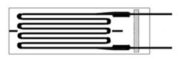
\includegraphics[width=.5\linewidth]{Assets/Biosignalverarbeitung-folien-dms.png}
  \end{itemize*}

  Dehnungsmessrosette:
  \begin{itemize*}
    \item Messung in drei Richtungen
    \item 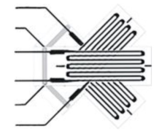
\includegraphics[width=.5\linewidth]{Assets/Biosignalverarbeitung-Dehnungsmessrosette.png}
  \end{itemize*}

  Wie man an diesen Konstruktionsbeispielen gut erkennen kann, bilden die
  Leitungen ungewollterweise eine Antenne, die alle vorhandenen Störungen
  aus der Umgebung aufnimmt, vor allem Netzeinstreuung, Mobilfunk und
  Computernetze.

  Aufbau von Massebezogenen und Massefreien Messungen:
  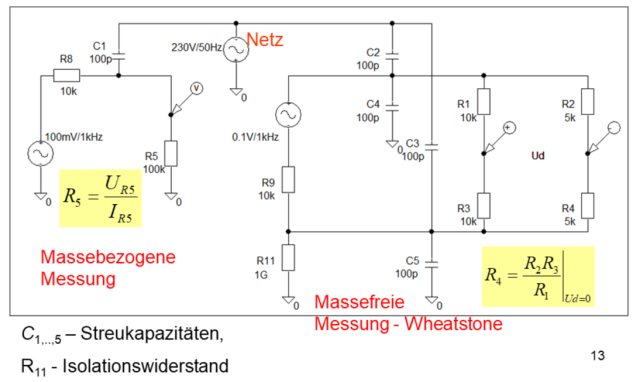
\includegraphics[width=.5\linewidth]{Assets/Biosignalverarbeitung-masse-messung.png}

  Messspannung von \$U\_\{R5\}\$ in der massebezogenen Schaltung
  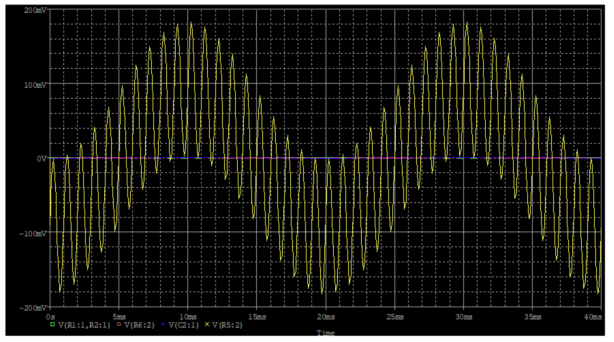
\includegraphics[width=.5\linewidth]{Assets/Biosignalverarbeitung-messspannung-massebezogen.png}
  Bei massebezogener Messung - auch Single-End genannt, da gegen Masse -
  werden die Störungen direkt dem Messsignal überlagert, so dass später
  eine Trennung ohne aufwendige Signalverarbeitung kaum möglich ist.

  Massebezogne eBrückenspannung (rot, blau) und Indikatorspannung \$U\_d\$
  (grün)
  \includegraphics[width=.5\linewidth]{Assets/Biosignalverarbeitung-massebezogen-brückenspannung.png}
  Einen großen Teil der Netzstörung bilden die elektrostatischen
  (kapazitiv eingekoppelten) Felder, die Gleichtaktcharakter haben. Diese
  lassen sich also durch Differenzbildung -hier mit einer Wheatstonschen
  Brücke -zum Teil eliminieren.

  \subsection{Durchfluss, Volumen}\label{durchfluss-volumen}

  \begin{itemize*}
    \item Massendurchfluss
    \begin{itemize*}
      \item \$\textbackslash dot m=\textbackslash frac\{dm\}\{dt\}\$
      \item \${[}\textbackslash dot m{]}=\textbackslash frac\{kg\}\{h\};\textbackslash frac\{g\}\{s\}
      \item industriell relevante Größe, z.B. Kraftstoffe, Luftverbrauch im Motor
    \end{itemize*}
    \item Volumendurchfluss
    \begin{itemize*}
      \item \$\textbackslash dot V=\textbackslash frac\{dV\}\{dt\}\$
      \item \${[}\textbackslash dot V{]}=\textbackslash frac\{m\^{}3\}\{h\};\textbackslash frac\{l\}\{min\}\$
      \item wichtige Messgröße in der medizinischen Messtechnik: Blutfluss, Atmung, Gastrointestinalapparat
    \end{itemize*}
    \item Der Durchfluss eines Mediums ist eine der wichtigsten Größen in der technischen und medizinischen Messtechnik. Technisch vor allem der Massendurchfluss, medizinisch der Volumendurchfluss, da medizinisch grundsätzlich die Volumina diagnostisch relevante Größe darstellen.
    \item Bei bekannter durchflossener Fläche wird der Volumenfluss über die Geschwindigkeitsmessung ermittelt
    \begin{itemize*}
      \item \$\textbackslash dot V=\textbackslash frac\{dV\}\{dt\}=\textbackslash frac\{A\emph{dl\}\{dt\}= A}v\$
      \item Reale Verteilung der Geschwindigkeit ist Parabel mit Maximum in der Mitte \$\textbackslash rightarrow\$ Gemessene Geschwindigkeit ist die mittlere Geschwindigkeit
    \end{itemize*}
    \item In der Medizin kann weder eine Geschwindigkeitsverteilung - wie in der Technik - erzwungen werden, noch kann sie vollständig erfasst werden. Daher misst man tatsächlich nur eine ,,mittlere'' Geschwindigkeit, wobei der Begriff ,,mittlere'' hier nicht ganz korrekt ist, da die tatsächliche Verteilung nach wie vor unbekannt ist.
    \item Messprinzip Druckdifferentmessung nach Gesetz von Hagen-Poiseuille
    \begin{itemize*}
      \item \$\textbackslash dot V=\textbackslash frac\{dV\}\{dt\}\textbackslash frac\{\textbackslash pi d\^{}4\}\{128\textbackslash mu\}*\textbackslash frac\{\textbackslash delta p\}\{l\}\$
      \item \$d\$ - Durchmesser der Kappilare
      \item \$\textbackslash delta p=p\_A - p\_B\$ - Druckdifferenz über der Kapillare, abhängigkeit von der Strömungsgeschwindigkeit
      \item \$l\$ - Länge der Kapilalre
      \item \$\textbackslash mu\$ - Viskosität des Mediums
      \item 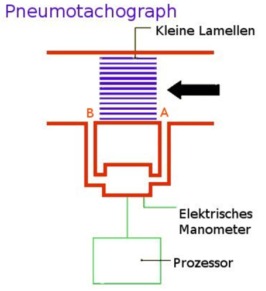
\includegraphics[width=.5\linewidth]{Assets/Biosignalverarbeitung-pneumotachograph.png}
      \item Bsp: 10\% Verengung der Kapillare \$\textbackslash rightarrow\$ 34\% Reduktion des Durchsatzes, d.h. im Blutkreislauf Anstieg des Blutdrucks um 34\%
      \item Bei externen Sensoren der Durchflussmessung kann man die Messbedingungen relativ klar vorgeben, z.B. im Pneumotachographen. Man erzwingt kapillare Strömung, der Strömungswiderstand und die Fläche sind bekannt, so dass aus der Druckdifferenz direkt auf den Durchfluss geschlossen werden kann.
    \end{itemize*}
    \item Anwendung in der Medizintechnik
    \begin{itemize*}
      \item Messung aller vitaler Lungenvolumina
      \item Messung des Blutflusses
    \end{itemize*}
    \item Nachteile des Messprinzips
    \begin{itemize*}
      \item zusätzlicher Strömungswiderstand verfälscht das Ergebnis
      \item bei Temperaturunterschieden Kappilaren-Medium Tröpfchenbildung
      \item geringer Dynamikbereich (1:10)
      \item niedrige Messgenauigkeit wegen Turbulenzen an Kapillarenden
      \item direkter Kontakt mit Medium
    \end{itemize*}
    \item Ultraschall-Geschwindigkeitsmessung nach dem Laufzeitverfahren
    \begin{itemize*}
      \item \$v=\textbackslash frac\{T\_2-T\_1\}\{T\_1 T\_2\}*\textbackslash frac\{L\}\{2\textbackslash{} cos\textbackslash{} \textbackslash alpha\}\$
      \item \$v\$ - mittlere Strömungsgeschwindigkeit des Mediums
      \item \$T\_1\$ - Laufzeit des Ultraschalls mit der Strömung
      \item \$T\_2\$ - Laufzeit des Ultraschalls gegen die Strömung
      \item \$L\$ - Länge des Ultraschall-Pfades
      \item \$\textbackslash alpha\$ - Winkel zwischen der Strömung und dem Ultraschall-Pfad
      \item 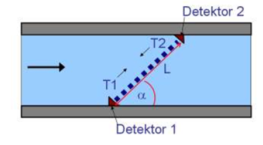
\includegraphics[width=.5\linewidth]{Assets/Biosignalverarbeitung-ultraschall-geschwindigkeit.png}
      \item Vorteile
      \begin{itemize*}
        \item kein Kontakt mit dem Medium, insbesondere Blutbahnen
        \item Installation und Messung ohne Unterbrechnung des Flusses
      \end{itemize*}
      \item Nachteile
      \begin{itemize*}
        \item invasive Methode, da Blutgefäß freigelegt werden muss
        \item Ungenauigkeit wegen der Verfomung der Blutgefäße
      \end{itemize*}
      \item Signaleigenschafte
      \begin{itemize*}
        \item verrauscht wegen Streuung im Medium, Sensorrauschen
        \item Echo statisch verteilt wegen Geschwindigkeitsprofil
      \end{itemize*}
    \end{itemize*}
    \item Ultraschall-Geschwindigkeitsmessung nach dem Dopplerverfahren
    \begin{itemize*}
      \item \$f\_D=f\textbackslash frac\{c\}\{c-v\} \textbackslash Rightarrow v=c\textbackslash frac\{f-f\_D\}\{f\_D\}\$
      \item \$c\$ - Ausbreitungsgeschwindigkeit des Ultraschalls im Medium
      \item \$f\$ - Originalfrequenz der Signalquelle
      \item \$f\_D\$ - gemessene Frequenz (Beobachter)
      \item \$v\$ - Geschwindigkeit der Signalquelle
      \item 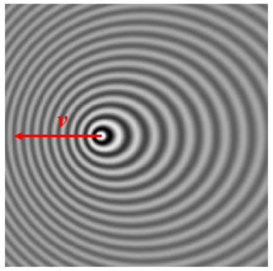
\includegraphics[width=.5\linewidth]{Assets/Biosignalverarbeitung-ultraschall-doppler.png}
      \item 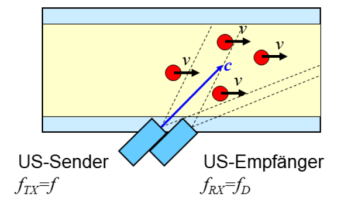
\includegraphics[width=.5\linewidth]{Assets/Biosignalverarbeitung-ultraschall-doppler-2.png}
      \item Anm: Feste Blutbestandteile (Blutkörperchen) reflektieren die Schallwellen und sind somit für den Ultraschall-Empfänger bewegte Signalquellen
    \end{itemize*}
    \item signalanalytisch relevante Eigenschaften
    \begin{itemize*}
      \item Flussgeschwindigkeit ungleichmäßig verteilt
      \item im technischen Bereich konstruktiv beherrschbar (Messkammer, Durchmesser, Material)
      \item im medizinischen Bereich kein Einfluss auf die Gefäße, daher relativ ungenaue Messung der mittleren Geschwindgkeit
    \end{itemize*}
  \end{itemize*}

  \subsection{Optische Sensoren}\label{optische-sensoren}

  Optische und Strahlungsquellen

  \begin{itemize*}
    \item Kaltlichtquelle: in der Endoskopie, bläuliches Tageslicht wegen der Farbtreue
    \item Diagnostische Laser: in der Ophthalmologie, Urologie, inneren Medizin, Dermatologie
    \item Leuchtdioden: in der Photoplethysomographie (Pulsoximetrie)
    \item Röntgen-, Gamma-, UV- und IR-Strahler: in der diagnostischen Bildgebung
    \item Inspektionslicht: in der HNO (Halogenstrahler)
  \end{itemize*}

  Signalanalytisch wichtige Eigenschafte

  \begin{itemize*}
    \item Temperaturstrahler: sind träge, daher statisches, konstantes Licht
    \item Halbleiter (Leuchtdioden), Laser und Leuchtstoffröhren sind gepulste Quellen - mit dem Auge nicht wahrnehmbar, aber analytisch unter Umständen sehr problematisch
  \end{itemize*}

  Optische Sensoren

  \begin{itemize*}
    \item Phototransistor: in Flachbilddetektoren der Radiologie
    \item Kamerachips: in den Endoskopen
    \item Szintillatoren: in Gamma-Kameras
    \item Photovervielfacher (SEV) in Laser-Fluroszenzsystemen
  \end{itemize*}

  Sensoreigenschaften

  \begin{itemize*}
    \item starkes Eigenrauschen, typisch für Halbleiter, ,,Dunkelstrom''
    \item hohe Temperaturabhängigkeit, ist materialbedingt, variable Parameter
    \item ungünstige Dynamikeigenschaften, Nachleuchten durch Trägheit, systemanalytisch lange Impulsantwort
  \end{itemize*}

  Beispiel Optischer Sensor CMOS Kamera LOGLUX i5

  \begin{itemize*}
    \item wahlfreier Pixelzugriff
    \item CameraLink oder FireWire Datenschnittstelle
    \item Auflösung 1280x1024 Pixel, 10 bit Graustufen
    \item \$\textgreater100\$ dB Kontrast-/Dynamikumfang
    \item ca 36 fps bei Vollbild; höhere Bildrate bei kleinerem Bildfeld bis ca 1500 fps
    \item Vorverarbeitung der Bilddaten mittels integrierter LUT (look-up-tables) möglich
    \item spektraler Arbeitsbereich 400-1000nm
  \end{itemize*}

  Optische Messmethoden gewinnen in der Medizin immer mehr an Bedeutung,
  vor allem, weil sie nichtinvasiv sind und daher patientenfreundlich. Mit
  der Kombination von Spektralfotometrie und Photoplethysmografie kann die
  Sauerstoffsättigung bestimmt werden. Dazu ist es notwendig, Gewebe
  durchzustrahlen, welches mit arteriellem Blut versorgt wird. Sehr
  verbreiten ist die Transmissionsmessung -d.h., das Gewebe wird
  durchstrahlt, was den Anforderungen an eine Messanordnung entsprechend
  der Theorie noch am nächsten kommt. Eine Alternative wurde notwendig, da
  der Finger u.U. nicht versorgt wird, z.B. beim Schock: Die
  Reflexionsmessung, bei der das Licht über einem Flächenknochen
  eingestrahlt und das reflektierte erfasst wird.

  \begin{itemize*}
    \item 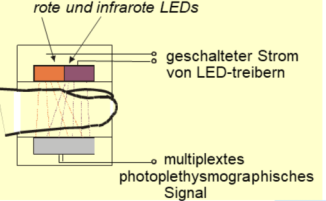
\includegraphics[width=.5\linewidth]{Assets/Biosignalverarbeitung-pulsoxy-1.png}
    \item 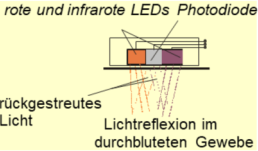
\includegraphics[width=.5\linewidth]{Assets/Biosignalverarbeitung-pulsoxy-2.png}
    \item 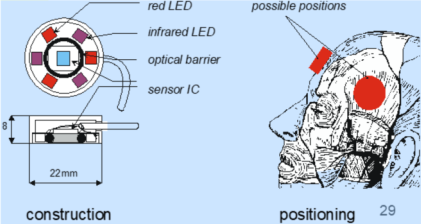
\includegraphics[width=.5\linewidth]{Assets/Biosignalverarbeitung-pulsoxy-3.png}
  \end{itemize*}

  Signal am Photodetektor

  \begin{itemize*}
    \item Multiplex bzw. sequentielle Abtastung
    \item Rauschen (Optoelektronik)
    \item Umgebungslicht, insbesondere Leuchtstoffröhren
    \item 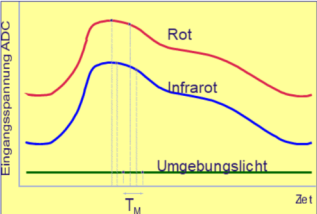
\includegraphics[width=.5\linewidth]{Assets/Biosignalverarbeitung-pulsoxy-4.png}
  \end{itemize*}

  Signal am Demultiplexer

  \begin{itemize*}
    \item DC ca 95-98\%
    \item AC nach DC Subtraktion verstärkt
    \item 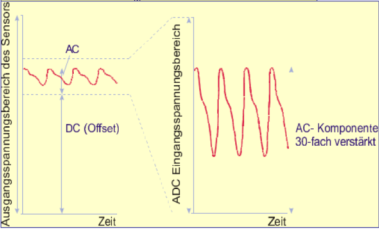
\includegraphics[width=.5\linewidth]{Assets/Biosignalverarbeitung-pulsoxy-5.png}
  \end{itemize*}

  Für die Signalverarbeitung bedeutet die Analyse des empfangenen Signals
  eine komplexe Herausforderung: Die Störungen, das Rauschen und das
  Umgebungslicht (vor allem im OP), sind enorm stark, so dass ihre
  Trennung vom Signal schwierig ist. Hinzu kommt, dass das Nutzsignal im
  unteren Prozentbereich des gesamten empfangenen Signals liegt, so dass
  hier das SNR um weitere zwei Dekaden schlechter wird.

  An diesem Beispiel eines realen Pulsoximetriesignals kann man die realen
  Eigenschaften erkennen:

  \begin{itemize*}
    \item 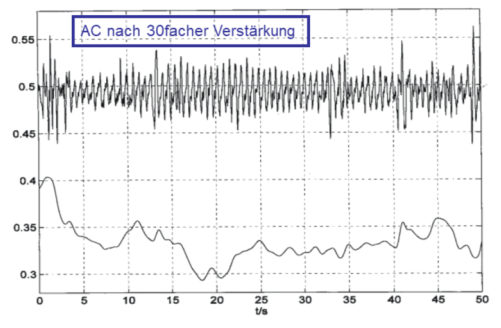
\includegraphics[width=.5\linewidth]{Assets/Biosignalverarbeitung-pulsoxy-6.png}
    \begin{itemize*}
      \item Der DC-Anteil, der im Grunde durch eine Tiefpassfilterung gewonnen wird, ist real ein stark schwankender gleitender Mittelwert (unterer Verlauf).
      \item Der AC-Anteil (oberer Verlauf) zeigt ebenfalls starke Schwankungen. Um dem Mediziner einen einigermaßen stabilen Messwert zu bieten, sind mehrere Schritte der SV notwendig
    \end{itemize*}
    \item 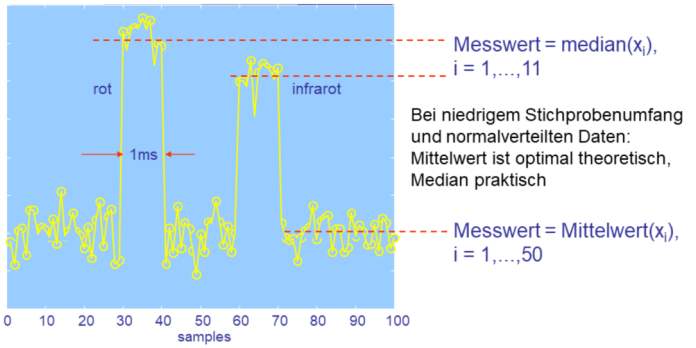
\includegraphics[width=.5\linewidth]{Assets/Biosignalverarbeitung-pulsoxy-7.png}
    \begin{itemize*}
      \item Pulsbreite 1ms, analoger Tiefpass 10kHz, Abtastrate 10 ksps
      \item Zunächst müssen aus dem Multiplexsignal die aktuellen Signalpegel für das rote und infrarote Licht sowie für das Umgebungslicht gewonnen werden: Durch die 10fache Überabtastung stehen für Rot und Infrarot zunächst elf Messwerte zur Verfügung. Dieser Umfang an Messdaten ist für eine Pegelbestimmung mit dem Mittelwert zu gering, daher wird der Median verwendet. Nach der Medianbildung liegen die Signalpegel für weitere Berechnung vor.
    \end{itemize*}
    \item 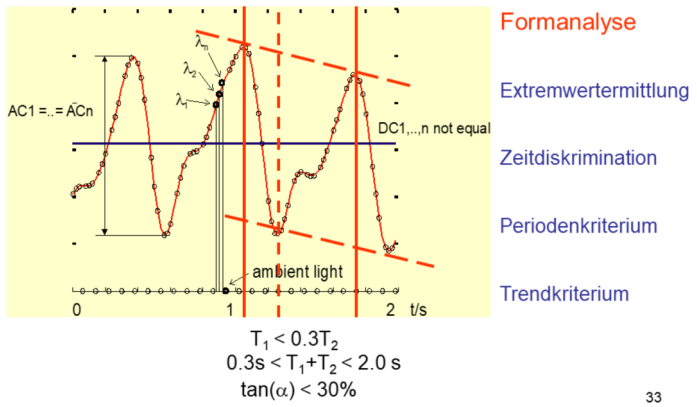
\includegraphics[width=.5\linewidth]{Assets/Biosignalverarbeitung-pulsoxy-8.png}
    \begin{itemize*}
      \item Die gewonnenen Signalpegel werden nun einer Signalanalyse unterzogen. Die Analyse bei einer Wellenlänge ist ausreichend, da die Signalform bei allen qualitativ identisch ist. Für die Bestimmung des AC-Pegels werden die Extrema detektiert. Aus der Physiologie ist bekannt, dass die Anstiegszeit der Pulswelle höchstens 30\% der Gesamtzeit beträgt, so dass eine Prüfung im Zeitfenster folgt. Weiterhin ist der Bereich der Periode bekannt, diese Prüfung folgt im nächsten Schritt. Durch Artefakte, vor allem durch Bewegung, entstehen Schwankungen der Basislinie. Nach einem empirische ermittelten Kriterium wird ein Trend von bis zu 30\% vor der Berechnung akzeptiert.
    \end{itemize*}
  \end{itemize*}

  \subsection{Akustische Sensoren}\label{akustische-sensoren}

  Physiologischer Schall (Herztöne, Atmungsapparat) liegt im hörbaren
  Bereich, so dass hier Methoden eingesetzt werden, die aus der
  allgemeinen Akustik bekannt sind. Konventionelle Mikrophontechnik mit
  spezifischer Signalverarbeitung

  \begin{itemize*}
    \item Verstärkung im tieffrequenten Bereich mit linearer Phase
    \item Richtcharakteristik umschaltbar bzw einstellbar, mechanisch bereits in den ältesten Stetoskopen
    \item spektrale Filterung für typische Geräusche, wie Herzklappen, Pfeifen in der Lunge, etc
    \item Merkmalserkennung in computerbasierter Auswertung, Mustererkennung typischer pathologisch bedingter Geräusche
  \end{itemize*}

  Beim Ultraschall (CW,PW,Doppler) handelt es sich um mechanische
  Schwingungen bis in den zweistelligen Megahertzbereich ( ca. 30MHz).
  Hier müssen aufwendige Methoden der SV angewandt und entwickelt werden,
  die primär -d.h. bis zum Übergang in den physiologischen Bereich bzw.
  zur Bildgebung -eher in der Nachrichtentechnik und Stochastik ihren
  Ursprung haben: Signaldetektion, Korrelationsrechnung, Histogramme,
  Signalzerlegung. Signalanalytisch wichtige Eigenschaften:

  \begin{itemize*}
    \item bei CW (Continous Wave) keine Tiefeninformation verfügbar, Information über Dopplerfrequenz mit hoher Variationsbreite, stochastischer Charakter mit viel Rauschen
    \item bei PW (pulsed Wave) Auflösung von der Signalverarbeitung entscheidend abhängig, da physikalische Grenzen lange erreicht
    \item in der Doppler-Technologie beides (CW und PW) vereint, daher Summe aller Vor- und Nachteile
  \end{itemize*}

  \subsection{Sensoren für elektrische Größen}\label{sensoren-fuxfcr-elektrische-gruxf6uxdfen}

  \subsubsection{Elektrochemische Grundlagen}\label{elektrochemische-grundlagen}

  \begin{itemize*}
    \item Dieser Sensortyp dient der Erfassung der elektrischen Aktivität des Menschen
    \item Der Mensch produziert elektrische Signale, daher ist keine Umwandung der Energieform notwendig
    \item Der Mensch ist elektrisch gesehen ein Volumentleiter der 2. Art - ein Elektrolyt oder ein Ionenleiter
    \item Das Messsystem ist mit metallischen Leitern aufgebaut - Leiter der 1. Art, Elektronenleiter
    \item daher ist die Schaffung einer Schnittstelle notwendig - die Elektrode
    \item 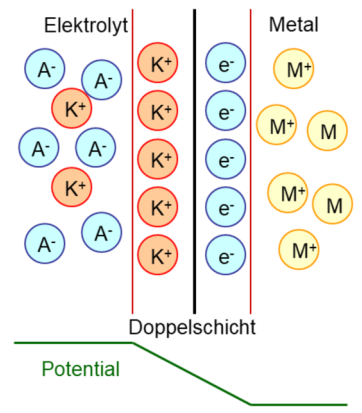
\includegraphics[width=.5\linewidth]{Assets/Biosignalverarbeitung-elektrochemische-grundlage.png}
    \begin{itemize*}
      \item \$mM \textbackslash Leftrightarrow mM\^{}+ + me\^{}-\$
      \item \$K\_k A\_a\textbackslash Leftrightarrow kK\^{}+ + aA\^{}-\$
      \item \$\textbackslash leftarrow\$: Reduktion; \$\textbackslash rightarrow\$: Oxidation
      \item Dynamisches Gleichgewicht an den Phasengrenzen
      \item An der Phasengrenze der beiden Leitertypen entwickelt sich -ähnlich wie in einem Halbleiter -eine Raumladungszone. Die freien Elektronen im Metall und die Kationen des Elektrolyts ziehen sich an und bilden an der Grenze eine Doppelschicht. Je nach der chemischen Zusammensetzung des Elektrolyts und des Metalls finden unterschiedlich starke chemische Reaktionen statt, die beim dynamischen Gleichgewicht die sog. Elektrodenspannung bilden. Funktionell handelt es sich hierbei also um ein ungewolltes Voltaisches Element.
    \end{itemize*}
  \end{itemize*}

  \subsubsection{Elektroden der Diagnostik}\label{elektroden-der-diagnostik}

  \begin{itemize*}
    \item aus signalanalytischer Sicht Eingangsdaten
    \item aus messtechnischer Sicht Systemeingang
  \end{itemize*}

  \begin{tabular}{l|l}
    Ziele                                 & Realisierbarkeit                                \\\hline
    geringe Elektrodenspannung            & durch Materialwahl (AgAgCl)                     \\
    geringer Drift der Elektrodenspannung & physiologisch bedingt, daher kaum beeinflussbar \\
    geringes Eigenrauschen                & Materialwahl und Technologie                    \\
  \end{tabular}

  Aus signalanalytischer Sicht sind die Ziele ganz klar vorgegeben. In der
  Praxis muss jedoch immer ein Kompromiss zwischen diesen Zielen und den
  Anforderungen der Anwendung und Praktikabilität gefunden werden: Wie
  diese Beispiele zeigen, hängt die Konstruktion der Elektrode von ihrer
  Bestimmung ab und daraus ergeben sich auch die Signaleigenschaften. So
  z.B. muss eine subkutane EMG-Elektrode die Form eine Nadel haben und aus
  einem Edelmetall sein. Dies hat zur Folge, dass die EMG-Elektroden
  relativ schlechte Signaleigenschaften aufweist: Riesige
  Elektrodenimpedanz (bis einige MOhm), stark kapazitives Verhalten, sehr
  hohe Elektrodenspannung (bis in den Voltbereich). Im Vergleich dazu
  haben die EKG-Elektroden -vor allem auf Grund ihrer großen Fläche und
  des Materials (AgAgCl, NaCl) -sehr günstige Eigenschaften: Niedrige
  Elektrodenimpedanz (kOhm-Bereich), sehr tieffrequent (bis DC), niedrige
  Elektrodenspannung (um 100 mV).

  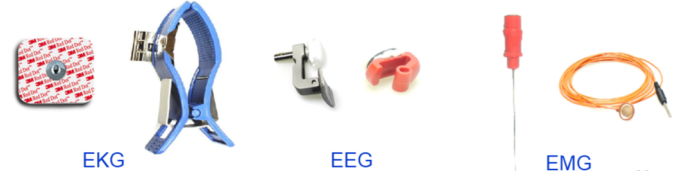
\includegraphics[width=.5\linewidth]{Assets/Biosignalverarbeitung-elektroden.png}

  \subsubsection{Elektroden der Therapie}\label{elektroden-der-therapie}

  \begin{itemize*}
    \item aus signalanalytischer Sicht Ausgangsdaten
    \item aus messtechnischer Sicht Systemausgang
  \end{itemize*}

  \begin{tabular}{l|l}
    Ziele                       & Realisierbarkeit                    \\\hline
    geringe Impedanz            & durch Materialwahl (beschichtet Cu) \\
    geringer Drift der Impedanz & physiologisch bedingt               \\
    Langzeitstabilität          & Materialwahl und Technologie
  \end{tabular}

  Ebensowichtig wie die Eigenschaften der diagnostischen Elektroden, sind
  es auch die der therapeutischen Elektroden. Dies liegt darin begründet,
  dass die Therapie von den zuvor analysierten diagnostischen Daten
  abhängt -natürlich im signalanalytischen Sinne, denn medizinisch ist es
  immer so. Man muss sich also bei der gewählten Therapie darauf verlassen
  können, dass das, was man auf die Elektrode schickt, so auch am
  biologischen Objekt ankommt. Diese Forderung technologisch umzusetzen
  ist ungleich leichter als bei diagnostischen Elektroden, denn hier
  können relative große Flächen mit gutem Kontaktmaterial verwendet
  werden.

  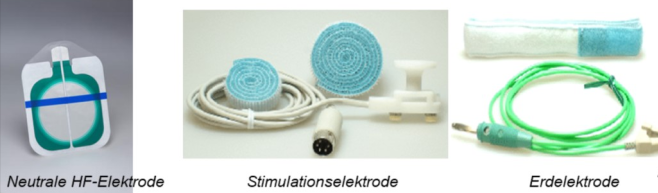
\includegraphics[width=.5\linewidth]{Assets/Biosignalverarbeitung-elektrode-therapie.png}

  \subsection{Sensoren für magnetische Größen}\label{sensoren-fuxfcr-magnetische-gruxf6uxdfen}

  \subsubsection{Messprinzipien}\label{messprinzipien}

  Um einen Eindruck über die Signalstärke (eher Signalschwäche) der
  biomagnetischen Signale zu bekommen, wird mit dem natürlichen Erdfeld
  verglichen, obwohl dieses für den Biomagnetismus eigentlich gar kein
  Problem darstellt. Störend sind die vom Menschen gemachten magnetischen
  Felder, vor allem die vom Stromversorgungsnetz, die jedoch weit über dem
  magnetischen Erdfeld liegen.

  \begin{enumerate*}
    \def\labelenumi{\arabic{enumi}.}
    \item Das stärkste Biosignal, das MKG, liegt 6 Dekaden unter dem Erdfeld (120dB), und weitere 2...3 Dekaden unter den technischen Feldern.
    \item MEG -7 Dekaden, oder 140dB,
    \item evozierte Felder -8 Dekaden oder 160dB
  \end{enumerate*}

  \begin{itemize*}
    \item \$10\^{}0T\$: MR-Tomographie-Magnete
    \item \$10\^{}\{-5\}T\$: Erdfeld
    \item \$10\^{}\{-6\}T\$: Zivilisationsfelder (Rauschen)
    \item \$10\^{}\{-9\}T\$: magn. Kontamination der Lunge
    \item \$10\^{}\{-10\}T\$: Magnetkardiogramm
    \item \$10\^{}\{-12\}T\$: Magnetoenzephalogramm
    \item \$10\^{}\{-13\}T\$: evozierte kortikale Aktivität
    \item \$10\^{}\{-15\}T\$: SQUID System Rauschen
  \end{itemize*}

  Biomagnetische Signale sind sehr schwach (SNR\textless{} -120dB).
  Mehrere Maßnahmen zur SNR-Anhebung notwendig

  \begin{itemize*}
    \item Abschirmung des Messkreises gegen Störfelder (dickwandige Kammer aus \$\textbackslash mu\$-Metallen)
    \item Ausnutzung der Feldeigenschaften - Gradiometer
    \item Spezialtechnologie der Signalverstärker - SQUID
  \end{itemize*}

  \subsubsection{Gradiometer}\label{gradiometer}

  Prinzip:

  \begin{itemize*}
    \item Störfelder meist ferne Quellen, Biologische Strukuren nahe Quellen
    \item ferne Quellen produzieren annährend homogenes Feld
    \item nahe Quellen Produzieren inhomogenes Feld
    \item mit Gradiometer wird die erste bzw zweite räumliche Ableitung gebildet, dadurch wird homogenes Störfeld unterdrückt
    \item 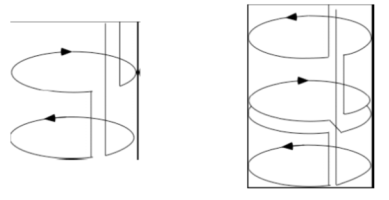
\includegraphics[width=.5\linewidth]{Assets/Biosignalverarbeitung-Gradiometer.png}
    \item 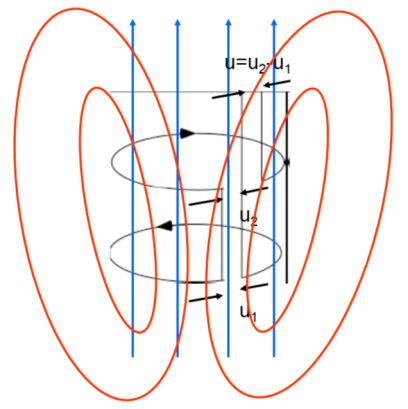
\includegraphics[width=.5\linewidth]{Assets/Biosignalverarbeitung-gradiometer-2.png}
    \item homogenes Fernfeld (Störung, blau): \$u=u\_2-u\_1=0\$
    \item inhomogenes Nahfeld (Biosignalquelle, rot): \$u=u\_2-u\_1\textless\textgreater0\$
  \end{itemize*}

  \subsubsection{SQUID}\label{squid}

  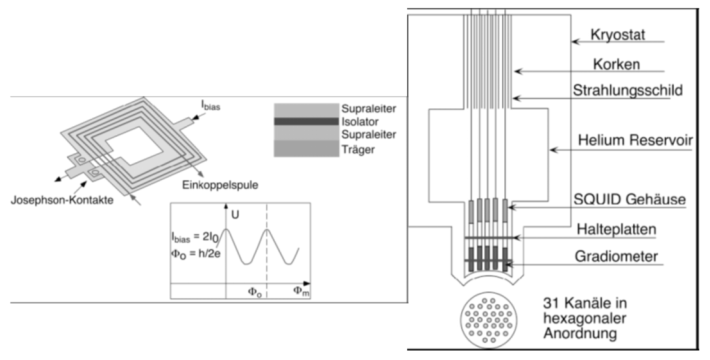
\includegraphics[width=.5\linewidth]{Assets/Biosignalverarbeitung-squid.png}

  Das supraleitende Quanteninterferenzgerät (SQUID) besteht aus zwei
  Supraleitern, die durch dünne Isolierschichten getrennt sind und zwei
  parallele Josephson-Kontakte bilden. Das Gerät kann als Magnetometer
  konfiguriert werden, um unglaublich kleine Magnetfelder zu erkennen -
  klein genug, um die Magnetfelder in lebenden Organismen zu messen. SQUID
  wurden zur Messung der Magnetfelder in Mäusehirnen verwendet, um zu
  testen, ob ihr Magnetismus ausreicht, um ihre Navigationsfähigkeit auf
  einen inneren Kompass zurückzuführen.
  \href{http://hyperphysics.phy-astr.gsu.edu/hbase/Solids/Squid.html}{Quelle}

  \section{Verstärkung und analoge Filterung}\label{verstuxe4rkung-und-analoge-filterung}

  \subsection{Eigenschaften von Biosignalen und Störungen}\label{eigenschaften-von-biosignalen-und-stuxf6rungen}

  \subsubsection{Entstehung der Biosignale, biologische Signalquellen}\label{entstehung-der-biosignale-biologische-signalquellen}

  \begin{itemize*}
    \item Analysegegenstand: Sensorisches, motorisches und zentrales Nervensystem
    \item Grundbaustein: Nervenzelle, Neuron. Einzelne Neurone kaum untersuchbar, im Einzelfall mit Mikroelektroden, dennoch für die Gesamtheit wenig Bedeutung. Wichtiger sind Untersuchungen an Neuronenverbänden und -strängen, z.B. motorische Steuerung von Muskeln in den Extremitäten. Hier haben die Nerven überschaubare und anatomisch sowie elektrophysiologisch gut bekannte Struktur.
    \item am Neuronausgang - Axon: Aktionspotentiale
    \item am Neuroneingang - Synapsen: EPSP/IPSP (exzitatorische und inhibitorische postsynaptische Potentiale)
    \item Sensorisches System ist deutlich komplexer, vor allem das akustische und das visuelle. So hat die Retina allein mehrere Millionen Sensoren (Stäbchen und Zapfen), die mit Ganglienzellen verbunden sind und bereits vor Ort relativ einfache Informationsverarbeitung durchführen.
    \item Zahlenmäßig und daher in auch in seiner Komplexität ist das größte das zentrale Nervensystem (ZNS), das aus ca. 10 Milliarden Neuronen besteht, die funktionelle und anatomische Zentren bilden aber zeitlich stark variierende Eigenschaften aufweisen.
    \item Signalanalytisch ist das Grundelement das Aktionspotential (AP), das vom Neuron nach Erreichen der Reizschwelle an seinen Eingängen über das Axon nach außen bzw. an andere Neurone abgegeben wird. Die Synapsen empfangen die Aktionspotentiale von anderen Neuronen und bewerten diese je nach Zustand mit EPSP oder IPSP, die von sich aus starken Veränderungen unterliegen. Im EEG sind die AP deutlich unterrepräsentiert (nur etwa 10\% des EEG), wesentlicher Anteil bilden die PSP. Dies ist unter anderem durch den Tiefpasscharakter des Schädels bedingt, das die hochfrequenten AP unterdrückt.
  \end{itemize*}

  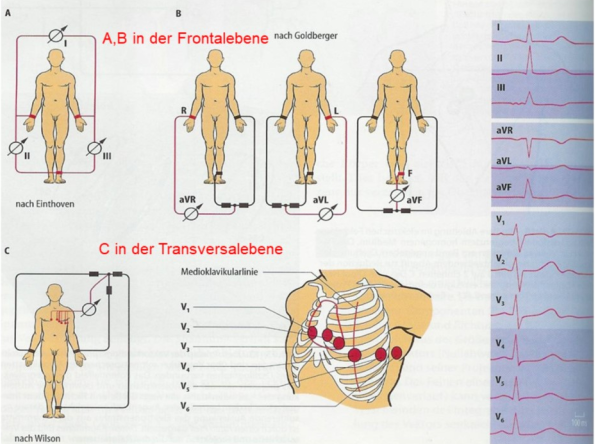
\includegraphics[width=.5\linewidth]{Assets/Biosignalverarbeitung-ekg.png}

  Ein medizinisch und auch signalanalytisch besonders interessantes Signal
  ist das EKG: Medizinische Indikation ergibt sich allein aus der
  besonderen Stellung des Herzens in der Physiologie als des Motors des
  Kreislaufs. Signalanalytisch ist es deswegen interessant, da es unter
  reproduzierbaren Messbedingungen (Extremitätenableitungen)
  formkonstanten Signalverlauf zeigt. Das EKG wurde entsprechend seiner
  elektromedizinischen Bedeutung extensiv untersucht, zahlreiche
  Erkrankungen und Schäden werden anhand typischer Formveränderungen des
  EKG diagnostiziert. Die Signalquelle des EKG ist das räumlich zwar recht
  komplizierte, aber anatomisch qualitativ konstante Reizleitungssystem
  des Herzens. Zur Ableitung des EKG werden standardmäßig 3-, 6-oder
  12-kanalige Extremitäten-und Brustwandsysteme verwendet.

  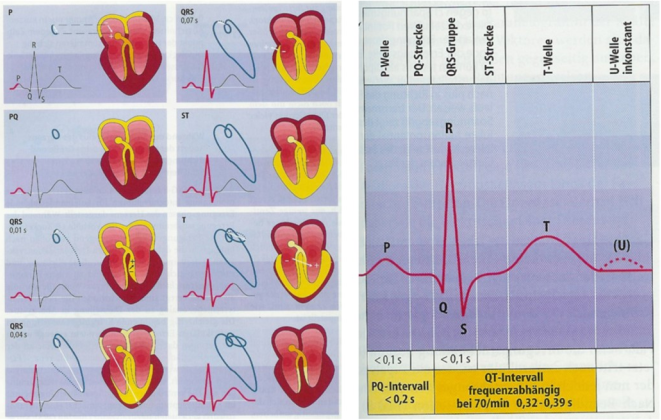
\includegraphics[width=.5\linewidth]{Assets/Biosignalverarbeitung-herz-ekg.png}

  Projektion der Reizausbreitung auf einen längs zur Herzachse liegenden
  Vektor (vertikal): Zu beachten ist, dass durch die Differenzbildung an
  zwei Punkten an der Körperoberfläche damit mathematisch die erste
  räumliche Ableitung (oder auch der erste Gradient) gebildet wird. Das
  hat zur Folge, dass die Ableitung nicht nur in Phasen der Ruhe (vor der
  P-Welle), sondern auch bei maximaler Erregung ( PQ-und ST-Strecke) Null
  ist. Wellen und Zacken im EKG sind Ausdruck der räumlich-zeitlichen
  Veränderung im Reizleitungssystem.

  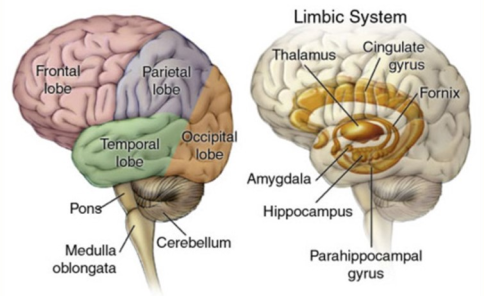
\includegraphics[width=.5\linewidth]{Assets/Biosignalverarbeitung-gehirn.png}
  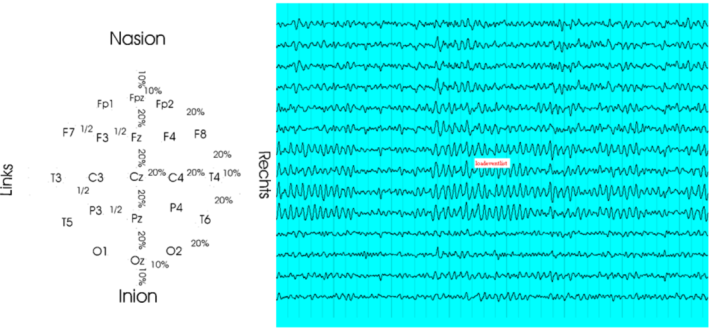
\includegraphics[width=.5\linewidth]{Assets/Biosignalverarbeitung-gehirn-ekg.png}

  Zur Ableitung des EEG werden wie beim EKG standardisierte
  Elektrodensysteme verwendet. Allerdings ist die anatomische Zuordnung
  hier ungleich schwieriger, denn die einzigen einigermaßen stabilen
  anatomischen Bezugspunkte sind das Nasion und das Inion. Es ist jedoch
  bekannt, dass die Lage des Gehirns in Bezug auf diese Punkte individuell
  stark unterschiedlich ist und im Zentimeterbereich liegt, so dass eine
  genaue Zuordnung der Elektroden zu Funktionszentren gar nicht möglich
  ist. Die Dichte der Elektroden in der Praxis liegt höchstens bei 10\%
  NI, d.h. im Schnit bei etwa 3cm. Eine höhere Dichte bringt keine
  zusätzliche Information, da der Schädel als räumlicher Tiefpass
  funktioniert und keine höhere Auflösung erlaubt.

  Aus Sicht der Signalanalyse ist es besonders wichtig zu wissen, unter
  welchen Messbedingungen das EEG abgeleitet wurde. Im Idealfall wird
  unipolar gegen verbundene Ohren oder Hals abgeleitet. Aus unipolaren
  Daten lassen sich die bipolaren Ableitungen einfach berechnen, umgekehrt
  geht das jedoch nicht. Auf jeden Fall ist zu klären, wie die
  Verschaltung des EEG-Verstärkers und der Elektroden realisiert wurde.
  Vermeintlich elegante Tricks, wie hardwaremäßige CAR sind auf jeden Fall
  zu meiden, ebenso Antialiasingfilter mit nichtlinearer Phase.

  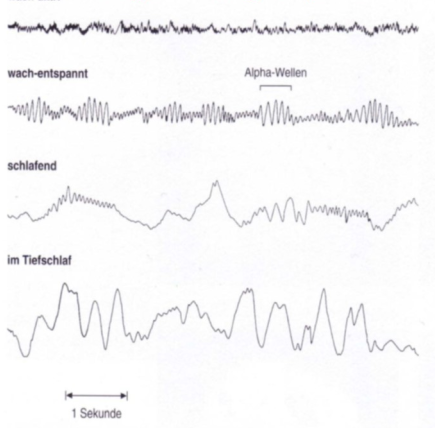
\includegraphics[width=.5\linewidth]{Assets/Biosignalverarbeitung-gehirn-eeg.png}

  Das EEG wird in in fünf typische Bereiche unterteilt: delta (0..4Hz),
  theta (4-7Hz), alpha (8..13Hz), beta (13..30Hz), gamma
  (\textgreater30Hz). Diese Bereiche sind typisch für bestimmte
  physiologischen (Schlaf, Konzentration, Entspannung) und pathologischen
  Bilder. Für die Signalanalyse ist wichtig, dass die Bereiche nicht
  gleichzeitig vorhanden sind, einer ist immer dominant, was die Analyse
  leicht vereinfacht.

  \subsubsection{Biologische und technische Störquellen}\label{biologische-und-technische-stuxf6rquellen}

  \begin{tabular}{l|l}
    periodische                       & transiente                \\\hline
    öffentliches Stromversorgungsnetz & Spannungsspitzen im Netz  \\
    Straßenbahn                       & Bewegungen im Messbereich \\
    Monitore                          & Schaltvorgänge            \\
    Kommunikationsnetze               & Lastschwankungen          \\
    Rotierende Maschinen              &                           \\
    Sender inkl. Funktelefon          &                           \\
  \end{tabular}

  1.Das biomedizinische Messsystem ist von vielen Störquellen umgeben, die
  meisten sind dem Bereich der Medienversorgung, Industrie, Verkehr und
  Nachrichtentechnik zuzuschreiben. Für die BSA sind periodische
  (Versorgungsnetz, Monitore) und quasiperiodische (rotierende Maschinen,
  Straßenbahn) Störungen noch ein vergleichsweise geringes Problem, denn
  diese lassen sich gezielt mit spektralen Filtern in der analogen
  Messkette oder digital nach ADC unterdrücken. 2.Wesentlich schwieriger
  ist die Situation, wenn transiente Störungen vorliegen, denn diese haben
  im Allgemeinen einen unbekannten, einmaligen und daher nicht
  reproduzierbaren Verlauf. Solange die transiente Störung die
  Signalerfassung nicht beeinträchtigt (durch Übersteuerung des
  Messverstärkers) und deutlich von der Signalform abweicht (z.B.
  Ausgleichsvorgang mi EKG), kann sie mit relativ einfachen Mitteln
  beseitigt werden, dennoch im Allgemeinen ist dies kaum möglich.

  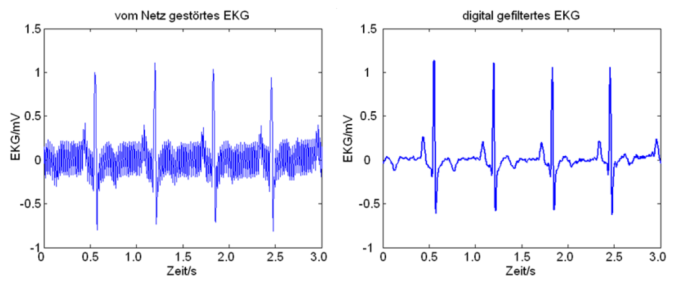
\includegraphics[width=.5\linewidth]{Assets/Biosignalverarbeitung-netzfrequenz-bandsperre.png}
  Die häufigste -weil immer vorhanden- ist die Netzstörung. Selbst
  batteriebetriebene portable Messgeräte sind von dieser Störung
  betroffen. Da die Frequenz der Störung aber bekannt ist, kann sie -falls
  keine Übersteuerung vorliegt- mit einer Bandsperre reduziert werden.
  Allerdings sollte nicht die früher übliche ,,50 Hz -Filter'' Taste
  verwendet werden, denn diese Filter haben einen nichtlinearen
  Phasenfrequenzgang und können das Biosignal deutlich verfälschen. Bei
  der heutigen Technologie werden ausschließlich digitale Filter
  verwendet.

  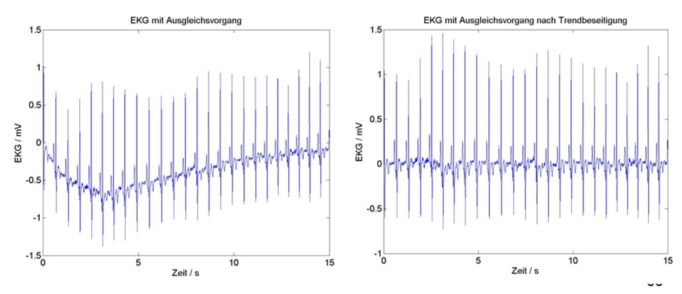
\includegraphics[width=.5\linewidth]{Assets/Biosignalverarbeitung-trendelimination.png} Eine
  sehr häufige transiente Störung im medizinischen Bereich ist die
  Bewegungsartefakte. Jegliche Bewegung im Messbereich erzeugt in der
  empfindlichen medizinischen Messtechnik Ausgleichsvorgänge. Wenn die
  Signalform gut bekannt ist, wie z.B. beim EKG, so lässt sich eine
  langsame Artefakte durch Hochpassfilterung beseitigen.

  \begin{itemize*}
    \item Maximal \$f\_\{0,01\}=0,5 Hz\$ Patienten-Monitor EKG (nicht oberhalb)
    \item Maximal \$f\_\{0,02\}=0,05Hz\$ Diagnostischer Monitor bei EKG (nicht oberhalb)
  \end{itemize*}

  Ob ein Biosignal gewollt ist oder eine Störung darstellt, ist von der
  Messaufgabe abhängig:

  \begin{itemize*}
    \item soll das EKG gemessen werden, ist das EMG eine Störung
    \item soll das EEG gemessen werden, ist das EKG eine Störung
    \item soll das EOG gemessen werden, ist das EEG eine Störung
  \end{itemize*}

  Prinzipielles Problem: Biologische Störquellen lassen sich nicht
  abschalten und kaum unterdrücken

  Aus Sicht der BSA gestaltet sich das Problem der Störungen wesentlich
  schwieriger als bei technischen Störungen. Erstens, die Biosignalquellen
  befinden sich innerhalb des Körpers, daher können sie weder abgeschirmt
  noch abgeschaltet werden. Zweitens, das biologische Signalspektrum ist
  für alle Biosignale in etwa gleich, streckt sich von 0 bis etwa 1kHz aus
  und weist ein Maximum bei etwa 100Hz auf. Daher können biologische
  Störsignale mit spektralen Filtern allein nicht beseitigt werden.

  Ein weiteres -messmethodisches -Problem besteh darin, dass man
  Biosignale nicht pauschal in Nutz-und Störsignale trennen kann. Es ist
  vielmehr die Messaufgabe, an Hand der man diese Klassifikation vornehmen
  muss.

  \paragraph{Eigenschaften technischer Störungen}\label{eigenschaften-technischer-stuxf6rungen}

  \begin{tabular}{l|l}
    periodische Störungen                                                                & transiente Störungen                                                \\\hline
    NF-magnetische Felder nicht eliminierbar durch Schirmung, erzeugen Differenzspannung & kaum eliminierbar, da Signalform unbekannt und nicht reproduzierbar \\
    NF-elektrische Felder gut beherrschbar, erzeugen Gleichtaktstörungen                 & bestenfalls Detektion möglich, Messdaten nicht korrigierbar         \\
    HF-Felder immer mehr vorhanden (Kommunikationsnetze), Abschirmung unwirtschaftlich   &                                                                     \\
  \end{tabular}

  \begin{enumerate*}
    \def\labelenumi{\arabic{enumi}.}
    \item Naturgemäß erzeugen niederfrequente magnetische Felder am Verstärkereingang Differenzspannungen, die direkt mit dem Biosignal überlagert werden, so dass sie mit der üblichen Verstäkertechnik nicht reduziert werden können. Hinzu kommt, dass auch eine Abschirmung nicht viel bringt, da in diesem Frequenzbereich mehrere 10- Zentimeter dicke Eisenplatten verwendet werden müssten, was in der Praxis nicht realisierbar ist. Da die niederfrequenten elektrischen (kapazitiv eingekoppelten) Störfelder Gleichtaktsignale sind, können sie zum Teil gut durch die Differenzverstärkertechnik reduziert werden. In immer höheren Maße stören hochfrequente Felder, vor allem aus dem Mobilfunk, Datennetzen, WLAN, Bluetooth, etc. Eine Abschirmung ist im normalen Praxisbetrieb unwirtschaftlich, so dass eine Reduktion der Störung allein durch Maßnahmen der EMV zu erreichen ist.
    \item Wie schon erwähnt, transiente Störungen sind im Grunde nicht beherrschbar, da sie eigentlich nicht bekannt und nicht vorhersehbar sind. Mit Methoden der BSA ist zum Teil ihre Detektion möglich, wenn z.B. der Messbereich oder das Spektrum des Biosignals nachweislich verlassen wird. Diese Detektion kann allerdings nur dazu genutzt werden, die beeinträchtigten Daten zu verwerfen, eine Korrektur ist nicht möglich.
  \end{enumerate*}

  \paragraph{Eigenschaften biologischer Störungen}\label{eigenschaften-biologischer-stuxf6rungen}

  \begin{itemize*}
    \item Spektral alle Biosignale im selben Band (0...100Hz)
    \item Nichtlineare Verkopplung der Biosignale verhindern Trennung mit herkömmlichen Methoden
    \item Kein Biosignal deterministisch und reproduzierbar
    \item Transiente bzw apperiodische und instationäre Biosignale nicht qualifizierbar
    \item Eine Trennung kaum möglich, bestenfalls eine Reduktion (z.B. Abschwächung des EMG im EKG)
  \end{itemize*}

  Das größte Problem bei der Reduktion von biologischen Störsignalen ist
  ihre funktionelle Verkopplung und physikalische Überlagerung im
  Volumenleiter Mensch. Die funktionelle Verkopplung (z.B. Einfluss der
  Atmung auf die Herzrate) ist nicht abschaltbar, ist nichtlinear und
  qualitativ unbekannt bzw. mit Methoden der BSA nicht beschreibbar.
  Außerdem sind die Verkopplungen in ihrer Komplexität weitgehend
  unerforscht und höchstens in Ansätzen dokumentiert.

  Man kann im Einzelfall den Einfluss eines Biosignals auf ein anderes zum
  Teil reduzieren. So z.B. ist bekannt, dass das EMG ein breitbandiges und
  vor allem hochfrequentes Signals ist, während das EKG seine Hauptanteile
  eher im niederfrequenten Bereich besitzt. Daher kann man den Einfluss
  des EMG mit einem relativ einfachen Tiefpass reduzieren, allerdings auch
  auf Kosten der Beeinträchtigung des EKG.

  \subsection{Medizinische Messverstärker}\label{medizinische-messverstuxe4rker}

  \subsubsection{Dynamik, Linearität}\label{dynamik-linearituxe4t}

  Messverstärker Anforderungen:

  \begin{itemize*}
    \item Linearität im Arbeitsbereich
    \item Linearer Phasenfrequenzgang
    \item Geringes Eigenrauschen
    \item Hohe Gleichtaktunterdrückung
    \item Übersteuerungsfestigkeit
  \end{itemize*}

  \begin{enumerate*}
    \def\labelenumi{\arabic{enumi}.}
    \item Mit Linearität im Arbeitsbereich ist die statische Linearität des Verstärkers gemeint, also die statische Beziehung zwischen der Ausgans-zu der Eingangsspannung \$U\_a/U\_e\$.
    \item Mit linearem Phasengang ist die dynamische Linearität gemeint, also die Erhaltung der Signalform bei der Verstärkung. Beim nichtlinearen Phasengang wird die Veränderung der Signalform fälschlicherweise auch als ,,lineare Verzerrung'' bezeichnet, wohl in Anlehnung an die nichtlinearen Verzerrungen im Arbeitsbereich.
    \item Das Eigenrauschen des Messverstärkers ist ein sehr wichtiger Parameter vor allem in der medizinischen Messtechnik, denn das Rauschen liegt im Bereich der zu messenden Signale im unteren Mikrovoltbereich. Ausgerechnet das 1/f-Halbleiterrauschen liegt dort, wo die Biosignale ihren wesentlichen Spektralanteil aufweisen.
    \item Wie schon erwähnt, ein wesentlicher Teil der beherrschbaren technischen Störungen bilden die Gleichtaktsignale. Daher wird von den Messverstärkern eine hohe CMRR gefordert, die nicht unter 100dB liegen sollte.
    \item Die Empfindlichkeit eines Verstärkers allein ist noch kein hinreichendes Kriterium. Ein medizinischer Verstärker muss übersteuerungsfest sein, damit er nicht schon beim ersten Defibrilationsimpuls oder bei der ersten OP mit HF-Gerät seine Dienste aufgibt. Und dies zu gewährleisten ist für die Elektroniker eine echte Herausforderung: Es gilt nämlich das Ziel, einen Verstärker aufzubauen, der im Mikrovoltbereich arbeitet, dennoch bei Spannungen von mehreren 100V (Defibrilation) oder HF-Leistungen (um 100W) nicht beschädigt wird und zeitnah seinen Arbeitsbereich wiederfindet.
  \end{enumerate*}

  \includegraphics[width=.5\linewidth]{Assets/Biosignalverarbeitung-Linearität-arbeitsbereich.png}

  Die Pegel der Biosignale sind gut bekannt, so dass den Arbeitsbereich
  des Verstärkers vorzugeben, kein Problem darstellt. So wird dieser
  Bereich für das EKG etwa zwischen - 5 und +5 mV liegen. Als Reserve bis
  zur Begrenzung sollte man mindestens 50\% des Arbeitsbereiches vorsehen.

  \subsubsection{Eigenrauschen}\label{eigenrauschen}

  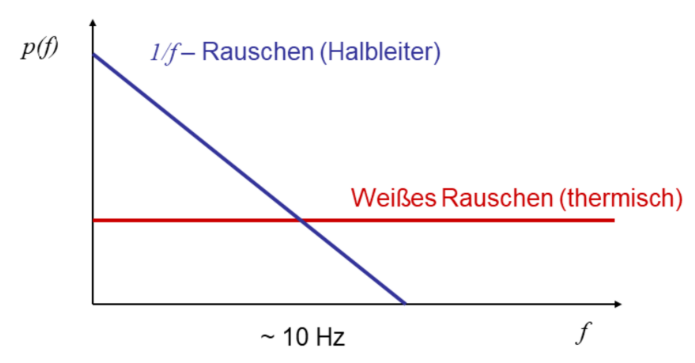
\includegraphics[width=.5\linewidth]{Assets/Biosignalverarbeitung-eigenrauschen.png}

  Das Halbleiterrauschen (1/f) erreicht bei etwa 10Hz den Pegel des weißen
  (Widerstands-) Rauschens. Da aber in diesem Bereich die meiste Energie
  der Biosignale liegt, ist es beim Schaltungsentwurf wichtiger, geeignete
  Halbleiter auszusuchen als sich auf die Minimierung des
  Widerstandsrauschens zu beschränken. Da die Auswahl an guten Halbleitern
  sehr begrenzt ist und dadurch den Entwicklern deutliche technologische
  Grenzen gesetzt sind, versuchen einige Konstrukteure und Hersteller die
  Eigenschaften ihrer Technik dadurch zu beschönigen, dass sie das
  Spektrum nach unten durch einen Hochpass begrenzen und erst dann die
  Rauschspannung messen und angeben. Daher muss man bei den Vergleichen
  verschiedener Techniken an dieser Stelle sehr vorsichtig vorgehen.
  Beispielsweise ist ein Verstärker, der angeblich nur 2uV Rauschspannung
  erzeugt aber erst bei 1Hz beginnt sicher nicht besser, als einer mit 3uV
  Rauschspannung dafür aber bereits ab 0.1Hz verstärkt.

  \subsubsection{Frequenzgang}\label{frequenzgang}

  Linearer Phasenfrequenzgang: Keine Formverzerrung

  \begin{itemize*}
    \item Gruppenlaufzeit: \$d(f)=const.\$
    \item Phasenfrequenzgang: \$\textbackslash phi(f)=\textbackslash int
  \end{itemize*}

  Die wichtigste Eigenschaft der Biosignale, die von Medizinern
  diagnostisch genutzt wird, ist ihre Signalform. Daher lautet eine der
  grundlegenden Anforderungen an die Messtechnik und die BSA, dass die
  Signalform nicht verfälscht werden darf. Das bedeutet, dass sowohl im
  analogen als auch im digitalen Teil des Messsystems die Gruppenlaufzeit
  konstant sein muss. Daraus lässt sich die Forderung herleiten, dass der
  Phasengang linear sein muss, zumindest im Übertragungsbereich.

  \subsection{Differenzverstärker}\label{differenzverstuxe4rker}

  \subsubsection{Funktionsprinzip}\label{funktionsprinzip}

  Vollkommene Symmetrie (DV und Signalanbindung)

  \begin{itemize*}
    \item \includegraphics[width=.5\linewidth]{Assets/Biosignalverarbeitung-Differenzverstärker-funktion.png}
    \item Vg ist Quelle der massebezogenen Störung. Die Störspannung gelangt auf beide Eingänge über Streukapazitäten, deren Impedanzen mit R4 und R5 simuliert werden, in gleicher Phase und im Idealfall auch mit gleichem Pegel. Die Störsignale an den Eingängen U10 und U20 sind also gleich, werden daher als Gleichtaktsignale bezeichnet.
    \item Vd ist die gewünschte massefreie Spannung (aus Sicht der Signalquelle zählen R4 und R5 nicht als Masseverbindung, die ,,hängt in der Luft'', floating source). Die Signalquelle Vd liegt direkt zwischen den Eingängen an, erzeugt daher eine Differenzspannung (siehe Funktionsprinzip eines Differenzverstärkers: Durch die Verkopplung der beiden Zweige T1 und T2 hat eine Zunahme der Eingangsspannung U10 Abnahme von Ud1 und Zunahme von Ud2, analog gilt das für U20. Daher liegt zwischen Ud1 und Ud2 die verstärkte Differenz von U10 und U20 an).
    \item Betrachtet man Ud1 und Ud2 massebezogen, so liegen überlagerte Gleichtakt- und Differenzspannungen an (unterer Grafik). Betrachtet man die verstärkte Spannung massefrei (also als Differenz zwischen Ud1 und Ud2), so verschwindet durch die Differenzbildung die Gleichtaktstörung und die gewünschte Differenzspannung bleibt übrig.
    \item Alle bisherigen Erläuterungen gelten nur im Idealfall: Sowohl der Verstärker ist ideal symmetrisch (identische Transistoren und Widerstände), als auch die Einkopplung der Gleichtaktstörung erfolgt ideal symmetrisch (über R4 und R5).
  \end{itemize*}

  Symmetrie im DV, asymmetrische (realistische) Signalanbindung

  \begin{itemize*}
    \item \includegraphics[width=.5\linewidth]{Assets/Biosignalverarbeitung-Differenzverstärker-asymmetrisch.png}
    \item In der Realität lassen sich zwar Verstärker bauen, die an das Ideal gut herankommen.
    \item Die Einkopplung der Gleichtaktstörung ist jedoch immer unsymmetrisch, es ist unmöglich, im Messkreis Symmetrie herzustellen (R4 und R5 unterschiedlich). Daher wird aus der ihrem Wesen nach Gleichtaktstörung zum Teil eine Differenzstörung. Und die Differenzstörung erscheint in der Ausgangsspannung Ud1-Ud2 zwangsläufig auch.
    \item Das heißt, in der Realität wird der Gleichtaktanteil der Störung zwar unterdrückt, aber der zur Differenz gewordene Anteil bleibt am Ausgang bestehen.
  \end{itemize*}

  \subsubsection{Differenz- und Gleichtaktverhalten}\label{differenz--und-gleichtaktverhalten}

  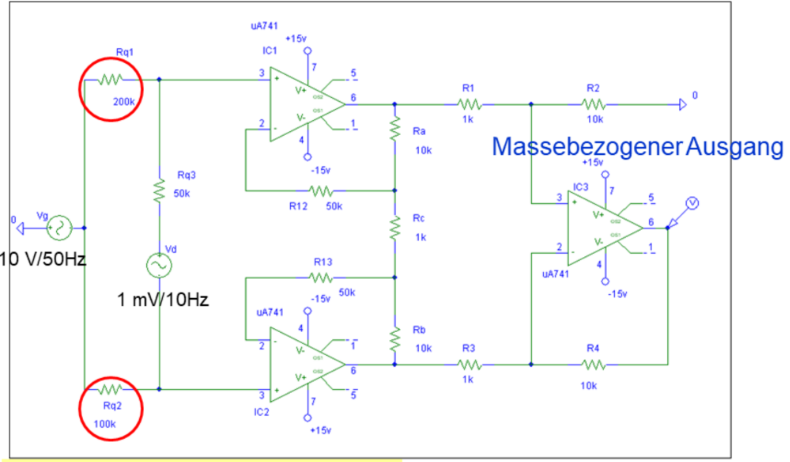
\includegraphics[width=.5\linewidth]{Assets/Biosignalverarbeitung-Diff-und-Gleichtakt.png}

  \begin{itemize*}
    \item \$SNR\_\{in\} = \textbackslash frac\{U\_\{d\_in\}\}\{U\_\{g\_in\}\}=\textbackslash frac\{1mV\}\{10V\}=10\^{}\{-4\}\textbackslash approx -80dB\$
    \item \$V\_g\$: Gleichtaktstörung (Netz)
    \item \$V\_d\$: Nutzsignal (EKG)
    \item Heute werden Differenzverstärker meistens als integrierte analoge Schaltungen mit OPVs eingesetzt. Da der Ausgang massefrei ist, folgt eine zweite Stufe zur Differenzbildung (IC3), die am Ausgang eine -wie üblich -massebezogene Spannung liefert. Diese Anordnung wird als Instrumentationsverstärker bezeichnet (instrumenation amplifier) und ist auch integriert verfügbar.
    \item Am Eingang liegt eine realistische Situation vor: Das gewünschte Signal hat den Pegel von 1mV (EKG), die Netzstörung erreicht (auch mehr als) 10V. Daher ist der SNR am Eingang sehr niedrig, -80dB.
    \item 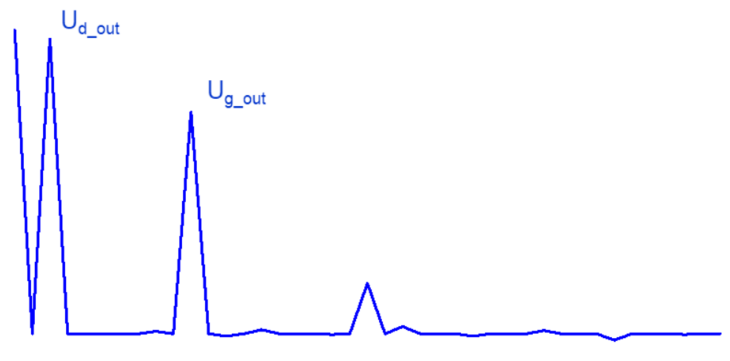
\includegraphics[width=.5\linewidth]{Assets/Biosignalverarbeitung-Diff-und-Gleichtakt2.png}
    \item \$CMRR=\textbackslash frac\{U\_\{d\_out\}\}\{U\_\{g\_out\}\}*\textbackslash frac\{U\_\{g\_in\}\}\{U\_\{d\_in\}\}=\textbackslash frac\{200mV\}\{20mV\} *\textbackslash frac\{10V\}\{1mV\}=10\^{}5\textbackslash approx 100dB\$
    \item Führt man mit dem Ausgangssignal des Verstärkers Spektralanalyse durch, so stellt man fest, dass die Netzstörung am Ausgang 20mV beträgt, während das gewünschte Signal 200mV erreicht, also der SNR am Ausgang ist 10 bzw. 20dB. Da der SNR am Eingang - 80dB betrug, wurde eine SNR-Verbesserung von 100dB erreicht. Diese Verbesserung ist auf die Gleichtaktunterdrückung selbst bei Asymmetrie am Eingang zurückzuführen, so dass in diesem Fall das CMRR identisch der SNR-Verbesserung ist. (Common-Mode Rejection Ratio, Gleichtaktunterdrückung, muss in der Medizintechnik laut Katalog mindestens 100dB, besser 120dB erreichen).
  \end{itemize*}

  \subsection{Instrumentationsverstärker}\label{instrumentationsverstuxe4rker}

  Der Instrumentationsverstärker (IV) ist ein mehrstufiger Verstärker, von
  dem in der medizinischen Messtechnik ein hoher Eingangswiderstand
  (besser als 100MOhm) und eine hohe CMRR (besser 100dB) gefordert wird.

  \subsubsection{Mehrstufiger Verstärker}\label{mehrstufiger-verstuxe4rker}

  \begin{itemize*}
    \item \includegraphics[width=.5\linewidth]{Assets/Biosignalverarbeitung-mehrstufiger-verstärker.png}
    \item Die erste Stufe ist der Eingangs-Differenzverstärker mit massefreiem Ausgang; die Ausgangsspannung ergibt sich aus der Differenz der Ausgangsspannungen von IC1 und IC2. Die zweite Stufe verstärkt zusätzlich und bezieht die verstärkte Spannung auf Masse, so dass am Ausgang massebezogene, verstärkte Eingangsdifferenz vorliegt.
    \item V1: \$u\_\{ad\}=A\emph{u\_\{ed\}+B}u\_\{eg\}\$, \$u\_\{ag\}=C*u\_\{eg\}+D+u\_\{ed\}\$,
    \begin{itemize*} \item \$A/B=F\$: Diskriminationsfaktor \item \$A/C=H\$: Rejektionsfaktor  \end{itemize*}
    \item V2:
    \begin{itemize*} \item \$u\_a=V\_d u\_\{ed\}+\textbackslash frac\{V\_d\}\{CMR\}u\_\{eg\}=V\_d(A u\_\{ed\}+\textbackslash frac\{A\}\{F\} u\_\{eg\})+\textbackslash frac\{V\_d\}\{CMR\}\textbackslash frac\{A\}\{H\} u\_\{eg\}\$ \item \$u\_a\textbar{}\emph{\{u}\{ed\}=0\} = V\_d A(\textbackslash frac\{1\}\{F\}+\textbackslash frac\{1\}\{CMR*H\}) u\_\{eg\}\$ \item die gesamt-Gleichtaktunterdrückung eines mehrstufigen Verstärkers ist abhängig im Wesentlichen von der ersten (Eingangs-) Stufe  \end{itemize*}
    \item Berechnet man die Ausgangsspannung in Abhängigkeit von der Eingangs-Gleichtaktspannung und von den Verstärkerparametern, so zeigt sich, dass für den CMRR die erste Stufe (wie auch bei anderen Parametern, z.B. Eigenrauschen) entscheidend ist, die folgenden Stufen sind unwesentlich beteiligt. Daher wird in der ersten Stufe der höchste Entwicklungsaufwand getrieben.
  \end{itemize*}

  \subsubsection{Hoher Eingangswiderstand}\label{hoher-eingangswiderstand}

  \begin{itemize*}
    \item 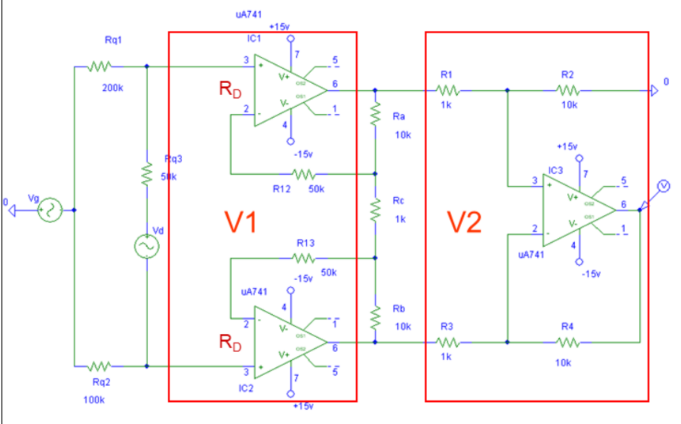
\includegraphics[width=.5\linewidth]{Assets/Biosignalverarbeitung-hoher-eingangswiderstand.png}
    \item \$R\^{}\{(1)\}\_\{ed\}=2R\_D+R\_C\textbackslash approx 2R\_D\$
    \item \$R\^{}\{(2)\}\_\{ed\}=R\_1+R\_3\textless\textless R\_D\$
    \item Theoretisch würde zur Ableitung von Biosignalen die zweite Stufe allein reichen, denn sie selbst verstärkt die Differenzspannung an ihrem Eingang (R1 und R3). Allerdings ist der Eingangswiderstand der zweiten Stufe für Biosignale viel zu niedrig. Eine zusätzliche Stufe mit hohem Eingangswiderstand ist daher notwendig, die außerdem noch wesentlich zur Verstärkung beiträgt.
  \end{itemize*}

  \subsubsection{Hohe Gleichtaktunterdrückung}\label{hohe-gleichtaktunterdruxfcckung}

  \begin{itemize*}
    \item \includegraphics[width=.5\linewidth]{Assets/Biosignalverarbeitung-hohe-gleichtaktunterdrückung.png}
    \item rot: OPs integriert
    \item blau: Widerstände getrimmt
    \item Gute Eigenschaften sind nur mit integrierter Technologie und getrimmten Widerständen erreichbar. Daher werden bis auf einige speziellen Ausnahmen ausschließlich integrierte IV eingesetzt.
  \end{itemize*}

  \subsection{Isolationsverstärker}\label{isolationsverstuxe4rker}

  Aus Sicherheitsgründen bzw. wegen zu hoher Spannungen ist es in der
  Medizin, aber auch z.B. in der Leistungselektronik, oft notwendig, den
  Messkreis von der Umgebung galvanisch zu trennen, ihn also bezugsfrei
  schweben zu lassen (floating circuit).

  \subsubsection{Funktionsprinzip}\label{funktionsprinzip-1}

  \begin{itemize*}
    \item \includegraphics[width=.5\linewidth]{Assets/Biosignalverarbeitung-Isolationsverstäker.png}
    \item Das Prinzip ist einfach: Alle Signalverbindungen und die Stromversorgung werden getrennt und entweder optisch oder transformatorisch über eine Isolationsbarriere realisiert. Da Biosignale sehr tieffrequent sind, müssen sie für die Übertragung moduliert bzw. demoduliert werden. Der Hardwareaufwand steigt enorm. Dennoch stehen heute bereits integrierte Isolationsverstärker zur Verfügung.
  \end{itemize*}

  \subsubsection{Galvanische Trennung und ihre Auswirkung}\label{galvanische-trennung-und-ihre-auswirkung}

  \begin{itemize*}
    \item 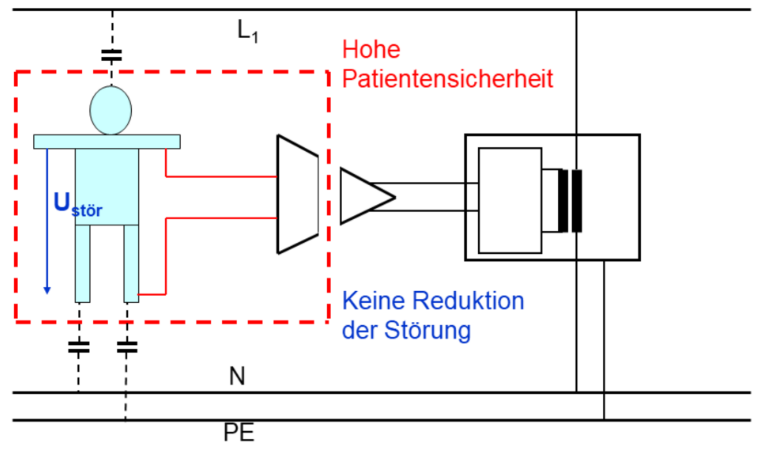
\includegraphics[width=.5\linewidth]{Assets/Biosignalverarbeitung-Galvanische-trennung.png}
    \item Durch die galvanische Trennung wird die Patientensicherheit enorm verbessert. Allerdings werden aus Sicht der Biosignalanalyse keine Verbesserungen erreicht, die Signaleingenschaften werden u.U. sogar noch schlechter. Der Grund sind die immer vorhandenen Streukapazitäten, die natürlich auch nach der galvanischen Trennung immer noch vorhanden sind und so Störungen in den Messkreis einkoppeln. Der notwendige Modem erzeugt weitere Störungen und Verzerrungen des gewünschten Signals.
  \end{itemize*}

  \subsubsection{Datenübertragung, Modulation und Demodulation}\label{datenuxfcbertragung-modulation-und-demodulation}

  \begin{itemize*}
    \item 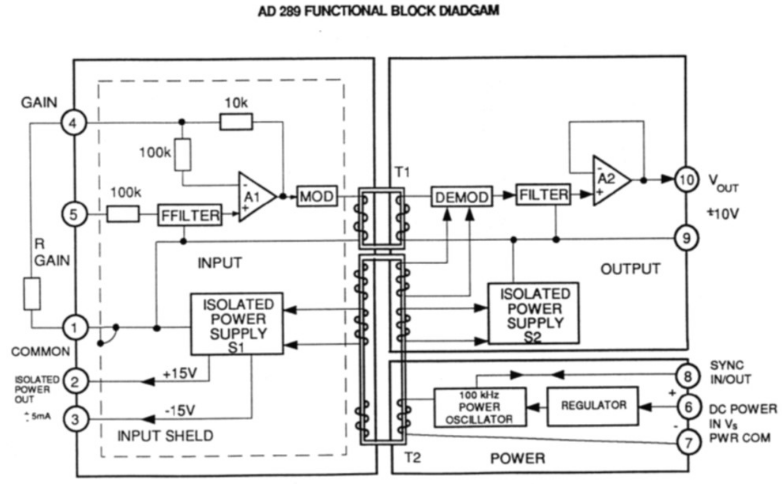
\includegraphics[width=.5\linewidth]{Assets/Biosignalverarbeitung-AD289.png}
    \item Realisierungsbeispiel von Analog Devices.
  \end{itemize*}

  \subsection{Guardingtechnik}\label{guardingtechnik}

  \subsubsection{Funktionsprinzip}\label{funktionsprinzip-2}

  \begin{itemize*}
    \item 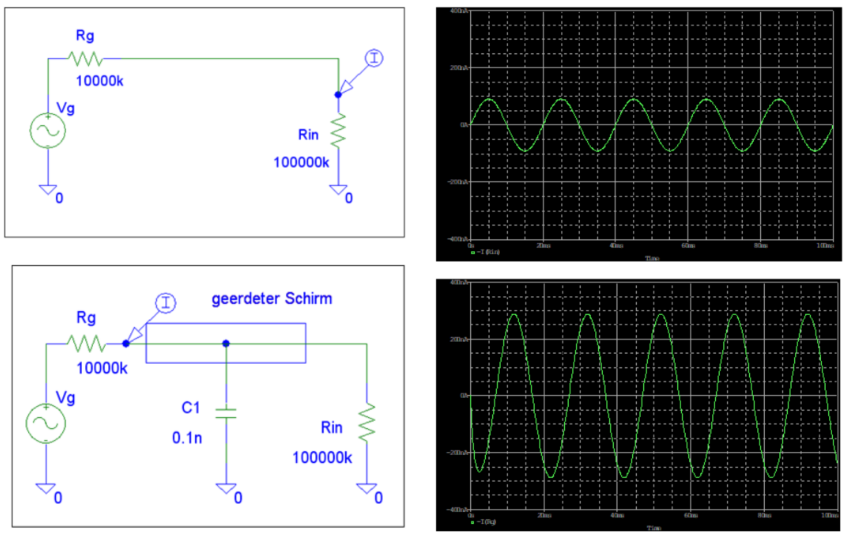
\includegraphics[width=.5\linewidth]{Assets/Biosignalverarbeitung-guarding.png}
    \item Eine wirkungsvolle Massnahme zur Störungsreduktion ist die Abschirmung der Messkabel, die in der Medizin bis zu zwei Metern Länge haben können (EKG) und damit gute aber unterwünschte Antennen realisieren. Der Schirm und das Messkabel bilden eine relativ große Kapazität von bis zu 100pF. Die Impedanz dieser Kapazität liegt parallel zum Eingangswiderstand des Verstärkers (untere Grafik) und reduziert diesen erheblich, wie man an den Verläufen des Messtromes erkennen kann: Während ohne Schirmung der Messstrom 100nA beträgt, steigt er auf 300nA bei Schirmung an, der Eingangswiderstand wurde also auf ein Drittel seines ursprünglichen Wertes reduziert und das ist inakzeptabel.
    \item 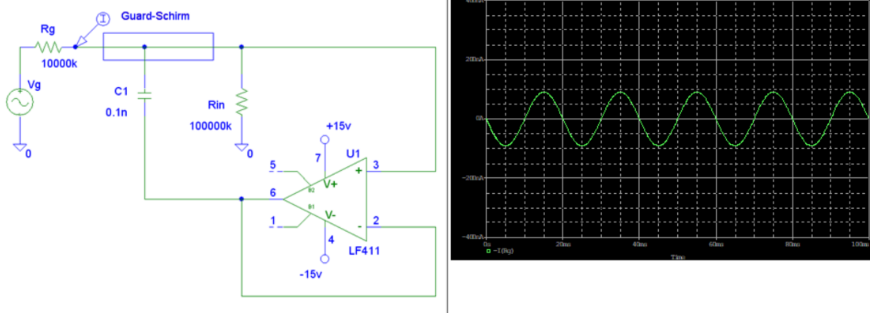
\includegraphics[width=.5\linewidth]{Assets/Biosignalverarbeitung-guarding2.png}
    \item Prinzip: Die Eingangsspannung wird über den Impedanzwandler an den Schirm gelegt. Die Schirmkapazität ist zwar immer noch vorhanden, über ihr liegt aber keine Spannungsdifferenz mehr an, also fließt auch kein Strom. Damit erscheint die Impedanz der Schirmkapazität vom Eingang her theoretisch unendlich groß, praktisch nah dran. Früher als Bootstrap-Prinzip bekannt.
    \item Die Impedanz der Kapazität wurde dynamisch idealerweise beseitigt, ist also theoretisch von den Eingangsklemmen nicht sichtbar. Die Kapazität ist aber nach wie vor physisch vorhanden! Diese Tatsache ist für bestimmte Fragestellungen sehr wichtig, z.B. Analyse bei implusartigen Störungen, bei den der Verstärker es natürlich dynamisch nicht schafft, den Impuls in Echtzeit auf den Schirm zu führen.
  \end{itemize*}

  \subsubsection{Realisierung}\label{realisierung}

  \begin{itemize*}
    \item 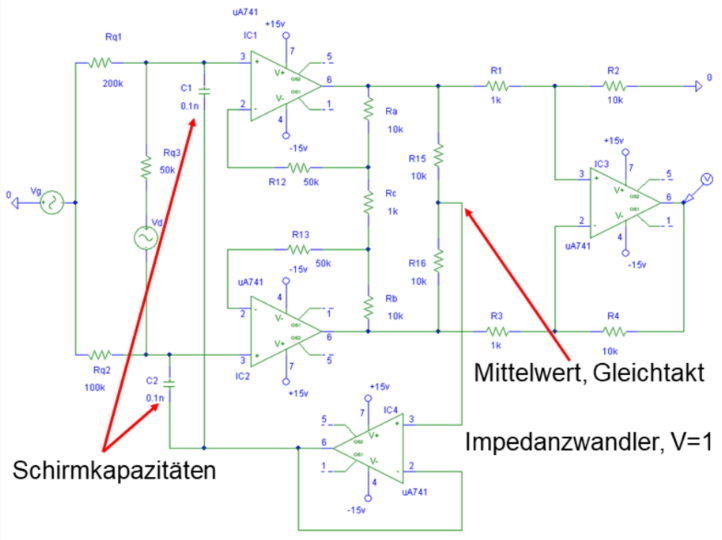
\includegraphics[width=.5\linewidth]{Assets/Biosignalverarbeitung-guarding-real.png}
    \item Schaltungstechnisch lässt sich Guarding mit einem zusätzlichen OPV (IC4) im IV realisieren. In diesem Fall wird nicht jeder Kanal einzeln, sondern alle mit dem Gleichtaktsignal belegt. Das spart Hardware und ist ausreichend, denn kritisch ist der Gleichtakt-Eingangswiderstand, während der Differenz-Eingangswiderstand nicht von Bedeutung ist.
  \end{itemize*}

  \subsection{Aktive Elektroden}\label{aktive-elektroden}

  \subsubsection{Funktionsprinzip}\label{funktionsprinzip-3}

  \begin{itemize*}
    \item 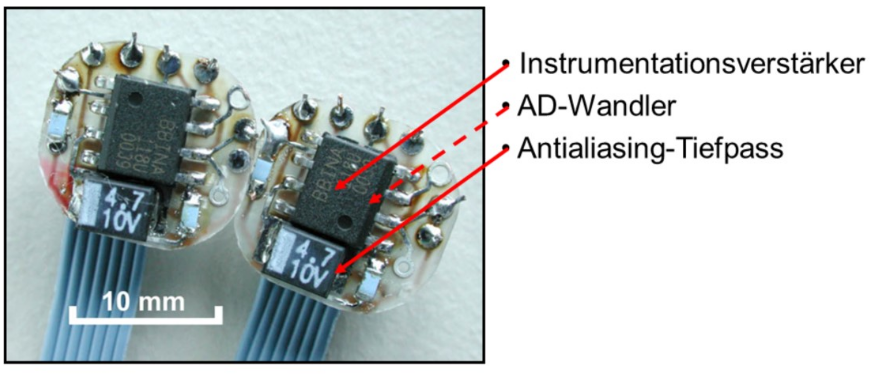
\includegraphics[width=.5\linewidth]{Assets/Biosignalverarbeitung-aktive-elektroden.png}
    \item Lösungsansatz: Verstärkung und Digitalisierung direkt auf Elektrode. Datenübertragung robust gegen Störungen, da binär
    \item Problem: Zuführung des Bezugspotentials notwendig
  \end{itemize*}

  \subsubsection{Störungsresistenz}\label{stuxf6rungsresistenz}

  \begin{itemize*}
    \item Aktive Elektroden technologisch aufwendig, haben aber Vorteile bei Störungen, die direkt auf die Messanordnung wirken
    \begin{itemize*}
      \item Elektrode: Drift der Polarisationsspannung kompensierbar
      \item Kabel: unempfindlich gegen kapazitiv, induktiv und HF-eingekoppelte Störungen
      \item Verstärkereingang: durch kürzste Wege zum Sensor keine direkte Beeinträchtigung der Eingangskreise
      \item Unsymmetrie: lässt sich in Rückkopplung computergesteuert reduzieren bzw. eliminieren
    \end{itemize*}
    \item die Übertragung ist digital, daher störungsresistent und distanzunabhängig
  \end{itemize*}

  \subsubsection{Gleichtaktunterdrückung}\label{gleichtaktunterdruxfcckung}

  Die unter 2.4.1 hergeleitete Gleichtaktunterdrückung gilt nicht
  pauschal, bei aktiven Elektroden ist Differenzierung notwendig

  \begin{itemize*}
    \item Aktive Elektroden meistens mit Verstärkung \$V=1\$
    \item daher CMR rechnerisch gleich 1, theoretisch zu niedrig
    \item prinzipbedingt starke Unterdrückung der Stör-Gleichtaktsignale
    \item daher praktisch sehr gute CMRR von 100dB und mehr
  \end{itemize*}

  \subsection{Analoge Filter}\label{analoge-filter}

  Das Unterscheidungskriterium ist, ob ein aktives Bauelement im Filter
  eingesetzt wird, d.h. ob es die Filtercharakteristik direkt beeinflusst.
  Dies ist der Fall bei allen rückgekoppelten Filtern mit Transistoren
  oder Operationsverstärkern. Dagegen ist ein Filter (z.B. RC-Tiefpass 1.
  Ordnung), dem ein OV als Impedanzwandler folgt, kein aktives Filter.

  \subsubsection{Passive Filter}\label{passive-filter}

  \paragraph{Grundlagen der Filtertheorie}\label{grundlagen-der-filtertheorie}

  \begin{itemize*}
    \item 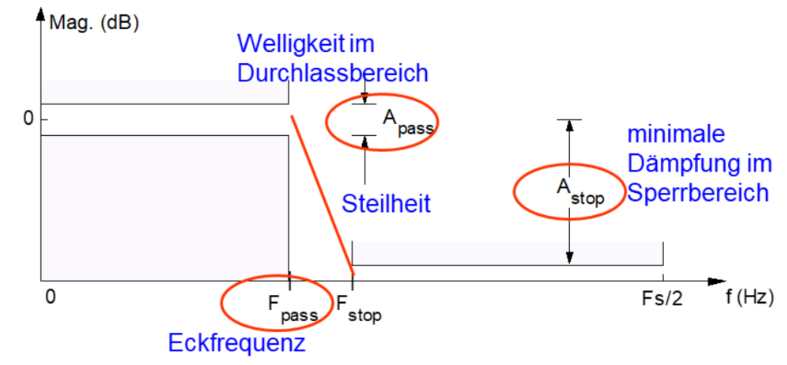
\includegraphics[width=.5\linewidth]{Assets/Biosignalverarbeitung-Filtertheorie.png}
    \item Bei spektralen Filtern werden folgende Parameter verwendet, um die Filtercharakteristik zu beschreiben:
    \begin{itemize*}
      \item Die Eckfrequenz, oder Grenzfrequenz: Frequenz \$F\_\{pass\}\$, bei der der Durchlassbereich in die Filterflanke übergeht und bei der die Übertragung um 3dB bzw. auf 70\% der Übertragung vom Durchlassbereiche abgesunken ist.
      \item Die Sperrfrequenz \$F\_\{stop\}\$, bei der die geforderte Dämpfung im Sperrbereich erreicht wird. Übergangsband Fstop-Fpass, auch transition band, ist der Übergangsbereich vom Durchlass-in das Sperrband, auch Filterflanke genannt. \item Steilheit ist Maß für die Filterflanke in dB/Hz. Grundsätzlich gilt, je steiler, umso besser. Hängt hauptsächlich von der Filterordnung ab.
      \item Welligkeit im Durchlassbereich Apass gibt an, im welchen Bereich die Übertragung im Durchlassbereich schwankt. Üblich ist weniger als 1dB, um 3dB ist für niedrige Ansprüche ausreichend.
      \item Minimale Dämpfung Astop gibt die garantierte Dämpfung an. Hängt hauptsächlich von der Filterordnung ab.
      \item Fs/2 ist die halbe Abtastrate oder die Nyquistfrequenz.
    \end{itemize*}
    \item 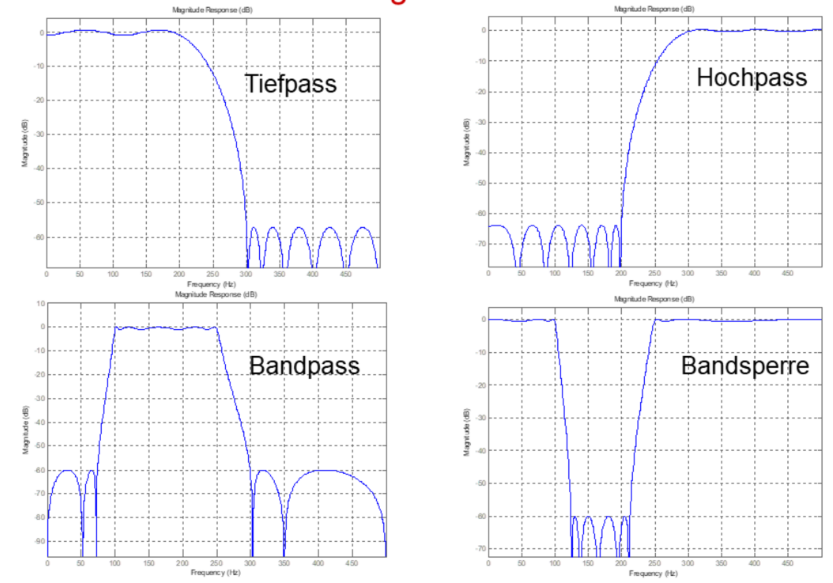
\includegraphics[width=.5\linewidth]{Assets/Biosignalverarbeitung-Filtertheorie2.png}
    \item Die Filtertheorie unterscheidet vier Grundtypen, siehe oben. Die Filtertheorie bietet ein Instrumentarium zum Entwurf von Filtern, vor allem aber für den nachrichtentechnischen Bereich, d.h. L-C-Kombinationen, also schwingfähige Systeme. Im Spektralbereich der Biosignale werden fast ausschließlich RC-Filter verwendet. Die Vorgehensweise beim klassischen Filterentwurf ist über die Schaltungsanalyse, also faktisch in einem Iterationsverfahren: Grundbausteine der spektralen Filter sind bekannt und mit diesen versucht man die gewünschte Charakteristik iterativ durch hinzufügen von Elementen und anschließender Analyse zu erreichen. Im analogen Bereich ist es kaum möglich, eine Filtercharakteristik vorzugeben und nach irgendeiner Methode die Schaltung als Ergebnis zu erhalten, der Entwurf ist daher sehr intuitiv und routineorientiert. Die Schaltungssynthese reduziert sich dann lediglich auf die Entnormung der Modelle auf konkrete Bauelemente.
    \begin{itemize*}
      \item Übertragungsfunktion \$G(j\textbackslash omega)=\textbackslash frac\{U\_2(j\textbackslash omega)\}\{U\_1(j\textbackslash omega)\}=\textbar G(j\textbackslash omega)\textbar*e\^{}\{j\textbackslash omega\textbackslash phi\}\$
      \item Amplitudenfrequenzgang \$\textbar G(j\textbackslash omega)\textbar=\textbackslash sqrt\{Re\{G(j\textbackslash omega)\}\^{}2 +Im\{G(j\textbackslash omega)\}\^{}2\}\$
      \item Phasenfrequenzgang \$\textbackslash phi(\textbackslash omega)=arctan\textbackslash frac\{IM\{G(j\textbackslash omega)\}\}\{Re\{G(j\textbackslash omega)\}\}\$
      \item Grenzfrequenz \$\textbackslash omega\_g=\textbackslash frac\{1\}\{RC\}\$
    \end{itemize*}
    \item Üblicherweise werden die Filter über ihre Übertragungsfunktion beschrieben, wobei auch äquivalente Beschreibungen möglich sind -Impulsantwort im digitalen Bereich, Pole-Nullstellen-Diagramme, seltener Zustandsgleichungen.
    \item Aus Sicht der BSA sind entscheidend die Beschreibungen über den Amplituden- und Phasenfrequenzgang.
  \end{itemize*}

  \paragraph{Filterentwurf}\label{filterentwurf}

  \begin{itemize*}
    \item passive Bauelemente
    \begin{itemize*}
      \item R,C,L
      \item mechanische Resonatoren
      \item Quarzfilter
      \item akustische Oberflächenwellenfilter
    \end{itemize*}
    \item im spektralen Bereich der Biosignale (0...1kHz) nur R und C
    \item Als Bauelemente zum Filterbau kommen neben R,C und L weitere Alternativen in Frage, die vor allem auf der mechanischen bzw. geometrischen Stabilität der schwingenden Anordnung aufbauen: piezokeramische und Quarzfilter oder akustische OWF.
    \item Im Spektralbereich der Biosignale kommen jedoch nur R-C-Kombinationen in Frage.
    \item Beispiele: oben ein zweikreisiger Parallelschwingkreis, der zur Schmalbandfilterung in der Nachrichtentechnik eingesetzt wird. Unten ein Phasenschiebernetzwerk, z.B. in einem RC-Generator.
    \begin{itemize*}
      \item 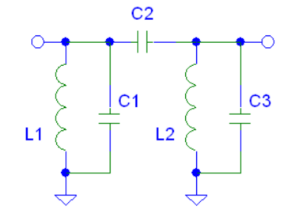
\includegraphics[width=.5\linewidth]{Assets/Biosignalverarbeitung-filterentwurf.png}
      \item \includegraphics[width=.5\linewidth]{Assets/Biosignalverarbeitung-filterentwurf2.png}
    \end{itemize*}
  \end{itemize*}

  \subsubsection{Aktive Filter}\label{aktive-filter}

  \begin{itemize*}
    \item \includegraphics[width=.5\linewidth]{Assets/Biosignalverarbeitung-tiefpass-2.ordnung.png}
    \item \includegraphics[width=.5\linewidth]{Assets/Biosignalverarbeitung-hochpass-2.ordnung.png}
    \item \$R\_\{0a\}=(\textbackslash epsilon-1)R\_0\$, \$u\_a=\textbackslash epsilon*u\_e\$ \$\textbackslash Rightarrow\$ Filtertyp mit \$R\_0\$ einstellbar \textbar{} \textbar{} Bessel \textbar{} Butterworth \textbar{} Tschebyscheff (1,5dB) \textbar{} \textbar{} -\/-\/-\/-\/-\/-\/-\/-\/-\/- \textbar{} -\/-\/-\/-\/-\/-\/- \textbar{} -\/-\/-\/-\/-\/-\/-\/-\/-\/-\/- \textbar{} -\/-\/-\/-\/-\/-\/-\/-\/-\/-\/-\/-\/-\/-\/-\/-\/-\/-\/-\/-\/- \textbar{} \textbar{} \$\textbackslash epsilon\$ \textbar{} \$1,267\$ \textbar{} \$1,586\$ \textbar{} \$2,482\$ \textbar{} \textbar{} \$\textbackslash gamma\$ \textbar{} \$0,618\$ \textbar{} \$1,0\$ \textbar{} \$1,663\$ \textbar{}
    \item Durch die Verwendung von OVs, die eine definierte Gegenkopplung ermöglichen, ist es mit relativ einfachen Mitteln möglich, effektive Filter zu konstruieren, die mit passiven Bauelementen allein um Größenordnungen komplizierter wären. Die beliebteste Entwurfstechnik ist die mit Hilfe von kaskadierten Stufen 2. Ordnung, auch im digitalen Bereich. Filter 2.Ordnung sind übersichtlich strukturiert, die Bauelemente müssen nicht mühsam ausgesucht und ausgemessen werden, die Eigenschaften sind sehr gut bekannt und bequem einstellbar, so dass eine kompliziertere Filterstruktur - z.B. Antialiasing-Tiefpass 8. Ordnung - durch einfache Kaskadierung (Serienschaltung) realisierbar ist. Natürlich muss man bei der Kaskadierung beachten, dass jede Stufe bei ihrer Grenzfrequenz 3dB-Abfall verursacht, so dass man die Kette entsprechend dimensionieren muss.
    \item Sehr vorteilhaft ist in dieser Schaltung, dass der Filtertyp bequem durch die Veränderung (Durchstimmung) eines einzigen Widerstandes über alle drei Basischarakteristiken eingestellt werden kann, sonst ist keine Veränderung der Schaltung notwendig.
    \item die Basistypen sind folgende:
    \begin{itemize*}
      \item Bessel, mit relativ flacher Flanke,
      \item Butterworth, mit wenig Welligkeit im Durchlassbereich, steilere Flanke als Bessel,
      \item Tschebysheff, mit steilster Flanke und Welligkeit im Durchlassbereich.
      \item \includegraphics[width=.5\linewidth]{Assets/Biosignalverarbeitung-aktive-filter.png}
      \item \includegraphics[width=.5\linewidth]{Assets/Biosignalverarbeitung-aktive-filter2.png}
      \item Bessel: niedrigste Flankensteilheit, konstante Gruppenlaufzeit
    \end{itemize*}
    \item Von allen drei hat nur Bessel konstante Gruppenlaufzeit, die in der BSA zwingend notwendig ist bei Echtzeitanwendungen. Folgen nichtkonstanter Gruppenlaufzeit sind u.a. Formverzerrungen, wie später gezeigt wird.
    \item \includegraphics[width=.5\linewidth]{Assets/Biosignalverarbeitung-diskreter-integrator-mit-ov.png}
    \begin{itemize*}
      \item \$\textbackslash tau=RC\$
    \end{itemize*}
    \item \includegraphics[width=.5\linewidth]{Assets/Biosignalverarbeitung-integrierter-integrator-mit-sc.png}
    \begin{itemize*}
      \item \$\textbackslash tau=\textbackslash frac\{1\}\{f\_S\}*\textbackslash frac\{C\_3\}\{C\_2\}\$
    \end{itemize*}
    \item Konventionell werden aktive Filter -am häufigsten der Antialiasing-Tiefpass vor dem AD-Wandler -mit Hilfe von OVs und RC-Netzwerken realisiert.
    \item Eine sehr elegante Alternative bieten die Filter mit geschalteten Kapazitäten: An Stelle des Widerstandes am Eingang befindet sich eine Kapazität, die im Takt von fs zwischen Eingang und dem OV umgeschaltet wird. Der mittlere Strom, der mit C3 integriert wird, hängt also von der Schaltfrequenz und dem Kapazität C2 ab. Daher ergibt sich die Zeitkonstante aus den beiden Kapazitäten, die auf dem Chip integriert sind und aus der Abtastfrequenz. Man kann also die Zeitkonstante allein durch Veränderung der Schaltfrequenz einstellen, ohne ein Bauelement der Schaltung ändern zu müssen.
    \item \includegraphics[width=.5\linewidth]{Assets/Biosignalverarbeitung-maxim7418.png}
    \begin{itemize*}
      \item Antianliasing-Tiefpass mit integriertem Filter 5. Ordnung
      \item kein RC-Netzwerk
      \item Grenzfrequenz abhängig nur vom Takt, daher durchstimmbar
      \item Eine Lösung für SC-Filter bietet u.a. Maxim, siehe oben. Die Kapazitäten sind allein zum Abblocken der Spannungsversorgung notwendig, für die Filterung selbst sind sie nicht notwendig.
      \item Der Takt muss den vorgeschriebenen Pegeln entsprechen, sonst ist es gleichgültig, aus welcher Quelle er geliefert wird.
    \end{itemize*}
  \end{itemize*}

  \subsection{Linearer Phasenfrequenzgang}\label{linearer-phasenfrequenzgang}

  \begin{itemize*}
    \item \includegraphics[width=.5\linewidth]{Assets/Biosignalverarbeitung-linearer-phasenfrequenzgang.png}
    \begin{itemize*}
      \item blau: das Eingangssignal
      \item rot: Ausgangssignal
      \item das Eingangssignal erscheint am Ausgang eines Tschebysheff-Filters wegen nichtkonstanter Gruppenlaufzeit verzerrt
    \end{itemize*}
  \end{itemize*}

  In vielen Bereichen der Technik (Nachrichtentechnik, Messdatenerfassung
  in Technik und Natur, Medizin) ist die Signalform der wichtigste
  Signalparameter. Daher ist es zwingend notwendig dafür zu sorgen, dass
  sie vom Messsystem nicht verzerrt wird. Notwendige, aber nicht
  hinreichende Bedingung für die Erhaltung der Signalform ist konstante
  Gruppenlaufzeit. Konstante Gruppenlaufzeit heißt, dass alle spektralen
  Anteile des Signals im System um gleiche Zeit verzögert werden. Ist
  diese Zeit nicht gleich, so erscheinen z.B. höherfrequente Anteil am
  Ausgang später als niederfrequente. Das obige Beispiel zeigt diesen
  Sachverhalt: Die Flanke eines Rechtecks ist ein zeitlich sehr schneller
  Vorgang, spektral demzufolge breitbandig von tiefen bis zu sehr hohen
  Frequenzen. Die hohen Frequenzen werden aber mehr verzögert als tiefe,
  was dazu führt, dass der Flanke am Ausgang hochfrequentes Nachschwingen
  folgt. Es wird demnach eine Signalform am Ausgang vorgetäuscht, die es
  am Eingang gar nicht gab.

  Die Form der Biosignale ist diagnostisch relevant, Formverzerrungen
  können zur falschen Diagnose führen

  \begin{itemize*}
    \item \includegraphics[width=.5\linewidth]{Assets/Biosignalverarbeitung-ekg-verzerrt.png}
    \item Der selbe Effekt tritt bspw. bei der EKG-Filterung mit einem Butterworth-Filter auf: Dieser Filtertyp besitzt einen nichtlinearen Phasenfrequenzgang, also nichtkonstante Gruppenlaufzeiten. Diese führen dazu, dass die hochfrequenten Anteile des QRS- Komplexes deutlich verspätet erscheinen, was in der Signalform schnelles Nachschwingen zur Folge hat. Dieser Effekt kann unter Umständen zur falschen Diagnose mit entsprechenden Folgen führen.
    \item \includegraphics[width=.5\linewidth]{Assets/Biosignalverarbeitung-ekg-verzerrt2.png}
    \item Das Original-EKG (schwarz) wurde mit einem IIR-Filter -das grundsätzlich einen nichtlinearen Phasengang hat -gefiltert und über das Original geschrieben (rot). Die relativ kurze Verzögerung der R-Zacke ist zunächst positiv und gewollt, damit das EKG in Echtzeit verarbeitet werden kann. Die Nachschwingungen nach der S-Zacke sind jedoch, wie beschrieben, sehr ungünstig.
    \item Das Spektrogramm des Original-EKG zeigt die ganz typische Energieverteilung in der t-f-Ebene: Die P-und T-Welle liegen im tieffrequenten Bereich bis ca. 10Hz. Die R-Zacke ist deutlich kürzer und hat Impulscharakter, so dass sie spektral wesentlich breiter ist und höhere Frequenzen beinhaltet, hier bis 50Hz, ohne Filterung bis 100Hz.
    \item Das Spektrogramm des gefilterten Signals (oben rechts) zeigt den typischen Effekt nichtkonstanter Laufzeit: Die Frequenzen(-gruppen), die höher als ca. 20Hz liegen, werden deutlich verzögert und erzeugen das schnelle Nachschwingen.
  \end{itemize*}

  \section{Signalkonditionierung, Abtastung und Digitalisierung}\label{signalkonditionierung-abtastung-und-digitalisierung}

  \subsection{Pegelanpassung}\label{pegelanpassung}

  Pegelanpassung notwendig für

  \begin{itemize*}
    \item massebezogene Eingänge von ADC (+/- 1V...+/-10V)
    \item standardisierte Schnittstellen (0...1V, z.B. Schreiber)
    \item verkabelte Übertragung zur Zentrale (Elektrodenbrause bei EEG)
  \end{itemize*}

  Realisierung mit

  \begin{itemize*}
    \item Pegelschieber
    \item programmierbare Verstärker (integierte analoge Elektronik)
    \item automatische Verstärkungsregelung (Rückkopplung)
  \end{itemize*}

  massefreie und massebezogene Signale

  \begin{itemize*}
    \item \includegraphics[width=.5\linewidth]{Assets/Biosignalverarbeitung-pegelanpassung.png}
    \item biologisches Objekt - Volumenleiter, immer kann nur Potentialdifferenz abgeleitet werden, d.h. massefrei (symmetrisch)
    \item bei der Verstärkung, spätestens bei der AD-Wandlung, Massebezug notwendig
    \item Wegen Störungen massefreie (symmetrische) analoge Strecke möglichst durchgängig bis zum ADC (verdrillte Leitungen, Differenzverstärker)
  \end{itemize*}

  \subsection{Abstastung, Aliasing}\label{abstastung-aliasing}

  Antastung im technischen Sinne ist die Erfassung des momentanen Wertes
  eines Signals zu definierten Zeitpunkten. Üblicherweise ist das Signal
  zeitkontinuierlich, nach der Abtastung liegt eine zeitdiskrete Variante
  des Signals vor

  \begin{itemize*}
    \item kontinuierliches Signal \includegraphics[width=.5\linewidth]{Assets/Biosignalverarbeitung-kontinuierliches-signal.png}
    \item zeitdiskretes Signal \includegraphics[width=.5\linewidth]{Assets/Biosignalverarbeitung-zeitdiskretes-signal.png}
  \end{itemize*}

  Abtastung ist mathematisch eine Multiplikation des Signals mit einer
  Folge von Dirac-Pulsen:
  \$y(t)=x(t)*\textbackslash sum\_\{n=-\textbackslash infty\}\^{}\{\textbackslash infty\}\textbackslash sigma(t-nT\_A)\$
  (\$T\_A\$ ist die Abtastperiode)

  Eine Multiplikation von zwei Signalen im Zeitbereich entspricht der
  Faltung ihrer Spektren im Frequenzbereich (und umgekehrt):
  \$Y(\textbackslash omega)=X(\textbackslash omega)*\textbackslash sum\_\{n=-\textbackslash infty\}\^{}\{\textbackslash infty\}
  \textbackslash sigma(\textbackslash omega-n\textbackslash frac\{1\}\{T\_A\})\$

  \includegraphics[width=.5\linewidth]{Assets/Biosignalverarbeitung-EKG-kontinuierlich-spektrum.png}

  \begin{itemize*}
    \item Das EKG ist natürlich digitalisiert, um es hier darstellen zu können. Die Abbildung entspricht jedoch einer Aufzeichnung unter realen Bedingungen.
    \item stark instationäres Signal mit scharfer R-Zacke. Daraus ergibt sich ein periodisches Spektrum, da die R-Zacke einen nahezu impulsartigen Verlauf hat. Beachten Sie die Beziehung zwischen impulsartigen Vorgängen in der Zeit und ihrem Spektrum.
  \end{itemize*}

  \includegraphics[width=.5\linewidth]{Assets/Biosignalverarbeitung-EKG-tasten-falten.png}

  \begin{itemize*}
    \item Um Überlappung (Aliasing) der Spektren und Mehrdeutigkeiten zu vermeiden, muss gelten: \$\textbackslash frac\{1\}\{T\_A\}\textbackslash geq 2*f\_\{max\}\$
    \item Nyquist-Frequenz entspricht der halben Grundfrequenz der Abtastrate, sie begrenzt nach oben das bei Null beginnende sog. Basisband. Das Basisband ist der Frequenzbereich, in dem man bei der Signalanalyse arbeitet. Damit das gespiegelte Spektrum nicht bis ins Basisband reicht und dadurch das Vorhandensein real nichtexistenter Signalkomponenten vortäuscht, muss gewährleistet werden, dass die halbe AR höher liegt, als die höchste Frequenz des Signals, d.h. die AR muss mindestens doppelt so hoch sein, die die höchste vorhandene Frequenz.
    \item Die periodische Wiederholung des Spektrums nach der Abtastung hat folgende praktische Bedeutung: Da sich das Spektrum mit jeder Harmonischen der AR wiederholt und gespiegelt wird, kann man ein bandbegrenztes Signal ins Basisband holen. So wäre bspw. denkbar, das zwischen 500 und 625 Hz liegendes EKG abzutasten und im Basisband zu verarbeiten. Dazu später ein Beispiel mit AM-modulierten EKG
  \end{itemize*}

  Ein aus Film und Fernsehen bekanntes Beispiel zur Verletzung des
  Abtasttheorems:

  \begin{itemize*}
    \item \includegraphics[width=.5\linewidth]{Assets/Biosignalverarbeitung-beispiel-film.png}
    \item Annahme: Ein Rad mit 8 Speichen dreht sich so, dass der Wagen sich mit 28.3 km/h bewegt, die Drehfrequenz des Rades beträgt demnach 2.5Hz. \$v=28,3\textbackslash frac\{km\}\{s\}=7,85\textbackslash frac\{m\}\{s\}\$, \$f=\textbackslash frac\{v\}\{U\}=\textbackslash frac\{7,85m/s\}\{3,14m\}=2,5Hz\$
    \item Die Periode, mit der die Speichen einen Referenzpunkt passieren (oben) beträgt 50ms bei einer Wiederholrate von 20/s \$f\_s=8*f=20Hz\textbackslash Rightarrow T\_s=50ms\$
    \item Entsprechend der Fernsehnorm werden 25 Bilder pro Sekunde aufgenommen, die Periode ist also 40ms. \$f\_A=25fps\textbackslash Rightarrow=40ms\$
    \item Entsprechend der Faltung beim Abtasten entstehen zwei Frequenzen -5 und 20, wobei nur die -5Hz im Basisband liegen. Das bedeutet praktisch, dass man das Rad langsam nach hinten drehen sieht. \$f\_\{SA\}=f\_A\textbackslash pm f\_S=-5/20 Hz\$
    \item reale Effekte: Räder (Auto), Stroboskopeffekt in Industriehallen mit Leuchtstoffröhren an rotierenden Maschinen
  \end{itemize*}

  \includegraphics[width=.5\linewidth]{Assets/Biosignalverarbeitung-rekonstruierter-sinus.png}
  Oft wird nach der Abtastung und anschließenden Signalverarbeitung das
  Ergebnis im ursprünglichen Bereich des Signals benötigt. Dazu ist die
  sog. Rekonstruktion notwendig, also eine Übertragung aus dem Analyse-in
  den Originalbereich. Zur Rekonstruktion ist allgemein eine Interpolation
  zwischen den diskreten Punkten notwendig, oder aus Sicht der
  Filtertheorie die Anwendung eines Interpolationsfilters. Das einfachste
  Interpolationsfilter ist ein Tiefpass in Nähe der höchsten
  Signalfrequenz. Wurde bei der Abtastung das Abtasttheorem verletzt, so
  treten im rekonstruierten Signal Komponenten auf, die im Originalsignal
  nicht vorhanden waren, siehe oben.

  Dieser Effekt kann auch im Fernsehen beobachtet werden: Tragen die
  Sprecher z.B. ein Hemd mit einem sehr feinen Strichmuster, so reicht die
  Bildschirmauflösung -d.h. die räumliche Abtastrate -nicht aus, um das
  Muster richtig zu erfassen und am Fernsehmonitor entsteht sog. Moiree,
  d.h. großflächige Farbmuster, die es in der Realität nicht gibt.
  \includegraphics[width=.5\linewidth]{Assets/Biosignalverarbeitung-abtastung-rekonstruktion.png}

  \begin{itemize*}
    \item \$y(t)=x(t)\emph{\textbackslash sum\^{}\{\textbackslash infty\}\_\{n=-\textbackslash infty\} \textbackslash sigma(t-nT\_A) \textbackslash Leftrightarrow Y(\textbackslash omega)=X(\textbackslash omega)}\textbackslash sum\^{}\{\textbackslash infty\}\_\{n=-\textbackslash infty\}\textbackslash sigma(\textbackslash omega-n\textbackslash frac\{1\}\{T\_A\})\$
    \item Übergang aus dem kontinuierlichen Zeitbereich in eine Folge, d.h. Entkopplung von der Abtastperiode
    \item \$y(n)=y(nT\_A) \textbackslash Leftrightarrow Y(k)=Y(k\textbackslash omega\_A/M)=\textbackslash sum\_\{n=1\}\^{}M y(nT\_A)\^{}\{-jkn/M\}\$
    \item \$Y(K)\textbackslash Leftrightarrow FFT(y(n))\textbackslash Rightarrow\$ normierte Frequenz \$\textbackslash omega\textbackslash in(0,2\textbackslash pi)\textbackslash vee f\textbackslash in(0,1)\$
    \item Nyquist Frequenz \$\textbackslash omega\_N=\textbackslash pi\$, \$f\_N=0,5\$
    \item Nach der Abtastung und Digitalisierung hat das Signal die Form einer Zahlenfolge bzw. eines Vektors oder Matrix. Ist die Abtastrate unbekannt, so ist das Signal auch nicht mehr reproduzierbar. Da sich aber Analysen und digitale Filterung grundsätzlich auch ohne Kenntnis der Abtastrate durchführen lassen, wird die sog. normierte Frequenz eingeführt, die bei der Rekonstruktion durch eine reale Abtastrate ersetzt wird.
  \end{itemize*}

  \includegraphics[width=.5\linewidth]{Assets/Biosignalverarbeitung-amplitudenmodulation.png}

  \begin{itemize*}
    \item \$EKG\_\{AM\}=EKG*sin(\textbackslash omega\_c t)\$
    \item Beispiel zum Abtasttheorem: Das EKG wird für eine Kabelübertragung mit einem Träger bei 10kHz multipliziert, was nachrichtentechnisch einer Amplitudenmodulation entspricht. Das Spektrum spiegelt sich um den Träger herum, ähnlich wie bei der Abtastung. Hier gibt es allerdings nur eine Spiegelung, da der Träger eine Harmonische ist und somit im Spektrum nur eine Nadel darstellt. Es entstehen zwei Seitenbänder, das obere und das untere. Beide sind hinsichtlich des Informationsgehaltes völlig identisch.
    \item Die Frage ist nun zu beantworten, wie hoch die Abtastrate für ein solches Signal sein muss.
  \end{itemize*}

  Abtasttheorem Kotelnikov, Channon (\$T\_A=1/2f\_\{max\}\$)

  \begin{itemize*}
    \item hinreichende/notwendige Bedingung
    \item hinreichend aber nicht notwendig \$AR\textbackslash geq 22ksps\$
    \item \$Y(\textbackslash omega)=X(\textbackslash omega)*\textbackslash sum\^{}\{\textbackslash infty\}\_\{n=-\textbackslash infty\} \textbackslash sigma(\textbackslash omega-n\textbackslash frac\{1\}\{T\_A\})\$
    \item notwendig und hinreichend: \$AR\textbackslash geq 2ksps\$
    \item \includegraphics[width=.5\linewidth]{Assets/Biosignalverarbeitung-abtastung-kotelnikov.png}
    \item Da die höchste Frequenz im Signal 11kHz beträgt, müsste die Abtastrate mind. 22ksps betragen. Dies ist eine hinreichende, aber keine notwendige Bedingung. Denn bezieht man sich auf die Wiederholung des Spektrums um jede Harmonische der Abtastrate, wird eine AR von 2ksps ausreichen. Damit passt eine Wiederholung des Spektrums in das Basisband, in wir ja analysieren.
  \end{itemize*}

  Pulsamplitudenmodulation (PAM)

  \begin{itemize*}
    \item nach Sample \& Hold
    \begin{itemize*}
      \item Zeit diskret
      \item Pegel analog
    \end{itemize*}
    \item \includegraphics[width=.5\linewidth]{Assets/Biosignalverarbeitung-Pulsamplitudenmodulation.png}
    \item Die Abtastung (sample \& hold) entspricht nachrichtentechnisch der PAM: die Werte treten in definierten Abständen entsprechend dem Pulsbreite (Abtastperiode) auf und haben einen kontinuierlichen Wertebereich. Allerdings spielt diese Modulationsart in der Nachrichtentechnik keine praktische Rolle, wichtig ist sie für die Theorie.
  \end{itemize*}

  Mehrkanalsystem - Simultansampling

  \begin{itemize*}
    \item \includegraphics[width=.5\linewidth]{Assets/Biosignalverarbeitung-Mehrkanalsysteme.png}
    \item Oft werden in der Technik und vor allem in der Medizin mehrkanalige Messsysteme benötigt. Für die Analyse ist von entscheidender Bedeutung, dass der zeitliche Zusammenhang der Kanäle identisch, oder zumindest bekannt ist. Beim echten Simultansampling werden alle Kanalsignale zum selben Zeitpunkt abgetastet und sequentiell digitalisiert. Damit reicht im Normalfall ein ADC für alle Kanäle.
    \item \includegraphics[width=.5\linewidth]{Assets/Biosignalverarbeitung-Mehrkanalsysteme2.png}
    \begin{itemize*}
      \item alle Kanäle im selben Augenblick abgetastet, echtes Simultansampling
    \end{itemize*}
    \item \includegraphics[width=.5\linewidth]{Assets/Biosignalverarbeitung-Mehrkanalsysteme3.png}
    \begin{itemize*}
      \item Um den HW-Aufwand zu minimieren, werden die Kanalsignale sequentiell abgetastet und digitalisiert, dabei kann die Einsparung an Elektronik beachtlich sein. Signalanalytisch kann sie jedoch problematisch sein: Aus der Signalsequenz wird das Simultansignal über die Laufzeitkorrektur in der FFT zurückgerechnet. Bei zeitkritischen Vorgängen ist diese Alternative zu verwerfen, da die durch die sequentielle Abtastung verlorengegangenen Signalteile durch Rückrechnung nicht mehr zu retten sind.
    \end{itemize*}
    \item \includegraphics[width=.5\linewidth]{Assets/Biosignalverarbeitung-Mehrkanalsysteme4.png}
    \begin{itemize*}
      \item Versatz der Kanäle um \$T\_A/N\$
      \item Rechnerische Korrektur der Abtastzeit (nicht-online-fähig)
      \item \$X\^{}*(j\textbackslash omega)=X(j\textbackslash omega)\^{}\{j\textbackslash omega T\_A/N\}\$
    \end{itemize*}
  \end{itemize*}


  \subsection{Digitalisierung}\label{digitalisierung}

  \subsubsection{Prinzipien der AD Wandlung}\label{prinzipien-der-ad-wandlung}

  Einrampenverfahren, Single-Slope-Conversion

  \begin{itemize*}
    \item \includegraphics[width=.5\linewidth]{Assets/Biosignalverarbeitung-Einrampenverfahren.png}
    \item Ur steigt aus dem negativen Bereich an, kreuzt es die Null, so wird K1 positiv. Da K2 noch positiv ist, da Ur unterhalb von Ue liegt, öffnet das Äquivalenzgatter = das Tor \& und der Zähler beginnt zu zählen.
    \item Erreicht Ur den Pegel von Ue, so wird K2 negativ bzw. logisch Null, = schließt und das Tor \& geht zu, der Zähler hört auf zu zählen. Der erreichte Zählerstand ist damit proportional der Spannung Ue.
    \item Vorteile: Einfach, wenig Aufwand, relativ schnell. Nachteil: stark temperaturabhängig, da Zählgrenzen von Analogwerten bestimmt. Wandelzeit abhängig von der Eingangsspannung.
  \end{itemize*}

  Zweirampenverfahren, Dual-Slope-Conversion

  \begin{itemize*}
    \item \includegraphics[width=.5\linewidth]{Assets/Biosignalverarbeitung-Zweirampenverfahren.png}
    \item In Phase 1 Aufladung durch die Eingangsspannung Ue über konstante Zeit. Damit ist der integrierte Wert proportional zur Ue.
    \item In Phase 2 Entladung mit konstanter Referenzspannung Ur bis zum Erreichen von Null. Damit ist die Entladezeit proportional Ue. Die Entladezeit wird digital gezählt, damit ist der Digitalwert am Ende proportional Ue.
    \item Vorteil: durch gespiegelte analoge Integration Temperatureinfluß weitgehend reduziert, da durch Auf-und Abintegrieren die Fehlerquellen mit entgegengesetzten Vorzeichen. Gute Genauigkeit von bis zu 16 bit. Nachteil: Wandlerzeit abhängig von Ue, daher nicht konstant.
  \end{itemize*}

  Sukzessive Approximation

  \begin{itemize*}
    \item \includegraphics[width=.5\linewidth]{Assets/Biosignalverarbeitung-Sukzessive-Approximation.png}
    \item Im Wesentlichen eine DA-Wandlung mit vorgeschaltetem Komparator. Macht Sinn, weil DA-Wandler präziser herstellbar als herkömmliche ADC.
    \item Prinzip: Das Steuerwerk beginnt mit dem MSB und schaltet die Bits bis zum LSB so lange um, bis die beste Approximation von Ue erreicht wurde, daher sukzessive Appr.
    \item Ablauf: ist bei MSB=1 die DAC-Spannung höher als Ue, so wird MSB=0 gesetzt, da der Komparator anzeigt, dass die DAC-Spannung zu hoch war. Ist bei MSB-1=1 die DAC-Spannung niedriger als Ue, so bleibt MSB-1=1 und das nächste Bit folgt. Es wird also sukzessive bis zum LSB nach der besten Annäherung gesucht.
    \item Vorteil: DAC technologisch präziser herstellbar als ADC. Konstante Wandlungszeit, daher planbar im Zeitregime. Gute Auflösung (bis 18bit), relativ schnell und preiswert.
  \end{itemize*}

  Delta-Sigma-Wandlung

  \begin{itemize*}
    \item \includegraphics[width=.5\linewidth]{Assets/Biosignalverarbeitung-Delta-Sigma-Wandlung.png}
    \item Beim Delta-Modulator handelt es sich um einen Ein-Bit-Wandler: Sobald das Eingangssignal x(t) die aufintegrierte bereits digitale Folge xD(t) über/unterschreitet, wird das Bit gesetzt/rückgesetzt. Damit erreicht man, dass das integrierte Binärsignal dem Eingangssignal mit höchstens einer Schrittweite als Fehler folgt.
    \item \includegraphics[width=.5\linewidth]{Assets/Biosignalverarbeitung-Delta-Sigma-Wandlung-2.png}
    \item Im Demodulator müssen die bei der Modulation durchgeführten Schritte invertiert werden: Der Integrator im Modulator wirkt insgesamt wegen der Rückführung differenzierend, so dass im Demodulator integriert werden muss. Wegen der Taktung muss im Demodulator noch ein Tiefpass folgen um das Signal zu glätten.
    \item Zwischen dem Modulator und dem Demodulator liegt die Übertragungsstrecke (Telemetrie, Multimedia, usw.). Unter der Annahme, dass sie linear ist, kann die Integration vom Demod nach vorn zum Mod vor den Summierer verlagert werden. Damit können beide Integratoren zu einem hinter dem Summierer zusammengefasst werden. Auf diese Weise entsteht der Delta-Sigma-Wandler (Differenz-Integration-1-Bit-Modulator).
    \item \includegraphics[width=.5\linewidth]{Assets/Biosignalverarbeitung-Delta-Sigma-Wandlung-3.png}
    \item Durch die Vorlagerung des Integrators reduziert sich der Demodulator (signalanalytisch) auf einen Tiefpass.
    \item \includegraphics[width=.5\linewidth]{Assets/Biosignalverarbeitung-Delta-Sigma-Wandlung-4.png}
    \item Diese Grafik zeigt die typischen Zeitverläufe im D-S-Modulator. Wie man bereits an der Blockstruktur erkennen konnte, handelt es sich -wie bei sukzessiver Approximation - um einen rückgekoppelten Kreis mit negativer Rückführung. In Anlehnung an die Regelungstechnik kann man demnach die Funktion so verstehen, dass die Bits im Bitstream so gesetzt werden, dass der Mittelwert des Ausgangs (siehe Integrator im Zeitverlauf) gegen Null bzw. einen Referenzwert läuft. Das digitale Ausgangssignal (Bitstream) ist qualitativ identisch mit eine Pulsbreitenmodulierten Signal, allerdings mit quantisiertem Pulsverhältnis. Das gleitende Mittel eines solchen Signals entspricht dem Originalsignal.
    \item Die erforderliche Taktrate ergibt sich aus der gewünschten Auflösung. So z.B. bei einer CD, die mit einer Abtastrate von 44,1kHz arbeitet und mit 16bit digitalisiert, kann der Takt des DS-Wandlers weit über 10MHz liegen (Oversamplingrate von 200).
  \end{itemize*}

  Flash-Converter, Parallelwandler

  \begin{itemize*}
    \item \includegraphics[width=.5\linewidth]{Assets/Biosignalverarbeitung-Parallelwandler.png}
    \item Am anderen Ende der Skala liegen die Flash-Converter. Diese sind sehr schnell, arbeiten weit in den Videobereich von über 100MHz hinein. Das geht natürlich nur auf Kosten der Parallelität, was bedeutet, dass für jede Quantisierungsstufe ein Komparator vorhanden sein muss. Für eine Bitbreite von 8bit werden also 256 Komparatoren benötigt. Dies ist heute integriert machbar aber auch schon die Obergrenze.
  \end{itemize*}

  \subsubsection{Breitbandige Wandler}\label{breitbandige-wandler}

  \includegraphics[width=.5\linewidth]{Assets/Biosignalverarbeitung-breitbandige-Wandler.png}

  \begin{tabular}{l|l}
    Resolution (Bits) & 24 bit                                      \\
    T-Put Rate        & 1kSPS                                       \\
    Kanäle            & 5                                           \\
    Supply V          & Single(+3), Single(+3.3), Single(+5)        \\
    Pwr Diss (max)    & 7mW                                         \\
    Interface         & Ser, SPI                                    \\
    Ain Range         & (2Vref/PGA Gain) p-p, Uni (Vref)/(PGA Gain) \\
    SNR (dB)          & 137dB                                       \\
    Pkg Type          & DIP, SOIC, SOP                              \\
  \end{tabular}

  \subsection{Telemetrie}\label{telemetrie}

  \subsubsection{Analoge Übertragung}\label{analoge-uxfcbertragung}

  \begin{itemize*}
    \item Direkt: verstärktes Signal auf kurze Entfernung, z.B. von der EEG-Brause zum Hauptverstärker
    \item Analoge Modulation über Kabel, z.B. EKG über Audiokarte im PC und Internet
    \item Analoge Modulation kabellos, z.B. Telemetriedaten von mobilen Patientenmonitoren (WLAN, Bluetooth, IR)
    \item \includegraphics[width=.5\linewidth]{Assets/Biosignalverarbeitung-analoge-übertragung.png}
    \item Das Prinzip der AM besteht darin, dass ein harmonischer Träger (Begriff der Nachrichtentechnik, das tragende Signal, die tragende elektromagnetische Welle) vom Modulationssignal so beeinflusst wird, dass seine momentane Amplitude dem Pegel des Modulationssignals entspricht.
    \begin{itemize*}
      \item Mathematisch und bei tiefen Frequenzen auch elektronisch einfach über Multiplikation des Trägers mit dem Modulationssignal realisierbar. Im HF-Bereich zur Ausstrahlung über Antenne über aufwendige Modulationsschaltungen und Leistungsverstärker.
      \item Das AM-Signal ist sehr störungsempfindlich, da Störungen direkt auf die Amplitude wirken, außerdem wird es als elektromagnetische Welle von aktuellen Ausbreitungsbedingungen beeinflusst. Für niedrige Ansprüche auf akustische Qualität akzeptabel z.B. Mittelwellen-Rundfunk oder Kurzwellen-Funk. Für Messtechnik als Trägermedium nicht geeignet. AM kann in ersten Stufen eines mehrkanaligen Systems eingesetzt werden (Untermodulatoren), in den keine Störungen von außen auftreten und welche die notwendige Bandbreite sehr sparsam nutzen im Vergleich zur FM
    \end{itemize*}
    \item \includegraphics[width=.5\linewidth]{Assets/Biosignalverarbeitung-analoge-übertragung-2.png}
    \item Im Spektrum des AM-Signals ist es sichtbar, dass die notwendige Bandbreite doppelt so groß ist wie die des Modulationssignals EKG. Diese ließe sich nochmal halbieren, also auf die ursprüngliche Bandbreite reduzieren, da das informationstragende Spektrum im AM-Signal doppelt vorhanden ist, daher auch die Bezeichnung DSB (double side band). Würde man z.B. die linke Hälfte wegfiltern, bliebe nur das eine zur Informationsübetragung notwendige Band übrig, daher die Bezeichnung SSB (single side band).
    \item \includegraphics[width=.5\linewidth]{Assets/Biosignalverarbeitung-analoge-übertragung-3.png}
    \item Bei der FM wird die Trägerfrequenz moduliert, d.h. die Momentanfrequenz des FM-Signals hängt vom aktuellen Pegel des Modulationssignals EKG ab. Wie die rechte Grafik zeigt, die Amplitude des FM-Signals ist konstant, die Dichte der Nulldurchgänge nimmt mit dem Pegel des Modulationssignals zu. Rechts ist in Zeitlupe der QRS-Komplex des EKG dargestellt (100ms der ersten Herzaktion aus der linken Grafik). Die hohe Amplitude der R-Zacke erzeugt im FM-Signal hohe Frequenzen (zwischen ca. 15ms und 65ms), während links und rechts der R-Zacke sichtbar tiefere Frequenzen vorliegen.
    \item Die FM ist besonders gut für Übertragungen sowohl kabelgebunden als auch kabellos (Telemetrieband 433MHz) geeignet, da sie sehr unempfindlich gegen Amplitudenstörungen ist -die Information ist allein in der Häufigkeit der Nulldurchgänge kodiert.
    \item \includegraphics[width=.5\linewidth]{Assets/Biosignalverarbeitung-analoge-übertragung-4.png}
    \item Ein wesentlicher Nachteil der FM ist die sehr hohe erforderliche Bandbreite des FM-Signals: diese beträgt das 10 bis 20-fache der Bandbreite des Modulationssignals. Beim EKG können daher Bandbreiten von bis zu 20kHz notwendig sein. Wie die rechte Grafik zeigt, erstreckt sich das Spektrum weit hinter die Nyquistfrequenz (2000Hz) aus, so dass man es vor der Abtastung mit einem Antialiasinftiefpass beschränken bzw. mit einer viel höheren Abtastrate abtasten müsste.
  \end{itemize*}

  \subsubsection{Digitale Übertragung}\label{digitale-uxfcbertragung}

  binäre Übertragung, PCM

  \begin{itemize*}
    \item \includegraphics[width=.5\linewidth]{Assets/Biosignalverarbeitung-digitale-übertragung-1.png}
    \item Die einfachste binäre Übertragung ist die PCM: nach Begrenzung des Spektrums nach oben bei 3.4 kHz bleibt ein Band von ca. 300 Hz bis 3.4 kHz übrig.
    \begin{itemize*}
      \item Nach der Abtastung mit 8 ksps liegt also ein zeitdiskretes wertanaloges Signal vor, entspricht der Puls-Amplituden-Modulation.
      \item Nach der AD-Wandlung mit 8 bit und P/S-Wandlung liegt ein serielles, binäres Signal vor, das PCM-Signal.
      \item Das PCM-Signal wird über Leistungsverstärker und Leitungsanpassung auf das Kabel gelegt, z.B. ISDN.
      \item Nicht eingezeichnet ist die Kompression, die die Dynamik des Sprachsignals begrenzt und die Reduktion der Bitbreite und damit der Übertragungskapazität ermöglicht.
    \end{itemize*}
    \item \includegraphics[width=.5\linewidth]{Assets/Biosignalverarbeitung-digitale-übertragung-2.png}
    \item Zur Übertragung über vorhandene Telefonkanäle ist es notwendig, die Pulse (z.B. der PCM) im Übertragungsband zur transportieren. Dazu werden der logischen Nullen und Einsen zwei verschiedene Frequenzen zugeteilt, die im Sender und im Empfänger gleich sind. Nach diesem Prinzip funktionieren die einfachen PC-Kommunikations-Modems.
    \item Natürlich kann man auch mehr Frequenzen zuweisen, z.B. mit 16 unterschiedlichen Frequenzen könnte man direkt Hexadezimalzahlen übertragen. Die rechte Grafik zeigt eine solche Alternative mit 16 verschiedenen Frequenzen (horizontal Zeit, vertikal Frequenz, Darstellung als Spektrogramm). Allerdings wurde hier das EKG nicht kodiert, sondern zur Veranschaulichung als 1-aus-16-Wert übertragen.
  \end{itemize*}

  Klassifikation digitaler Filter nach ihrer Impulsantwort als LTI-System
  (Linear Time Invariant)

  \begin{itemize*}
    \item IIR (Infinite Impulse Response)
    \begin{itemize*}
      \item Funktionales Äquivalent zu analogen Filtern
      \item Im allg. nichtlinearer Phasenfrequenzgang
    \end{itemize*}
    \item FIR (Finite Impulse Response)
    \begin{itemize*}
      \item Filtertypen realisierbar, die es in der analogen Welt nicht gibt (Hilbert, Allpass, adaptive Filter)
      \item Linearer Phasenfrequenzgang realisierbar
    \end{itemize*}
  \end{itemize*}

  Die Klassifikation nach der Länge der Impulsantwort (IR) orientiert sich
  allein nach praktischen Gesichtspunkten.

  \begin{itemize*}
    \item Durch die rekursive Struktur der IIR-Filter ist deren Impulsantwort (IR) nicht nur theoretisch, sondern auch praktisch unendlich lang. IIR werden auf Grund ihrer Struktur auch Rekursivfilter genannt. IIR haben eine sehr interessante Eigenschaft:
    \begin{itemize*}
      \item Rein theoretisch -und mit entsprechender Genauigkeit vielleicht auch praktisch -wäre damit ein unendlich langer Datenspeicher eines Zeitverlaufs realisierbar, denn der letzte Wert am Filterausgang reicht immer aus, um den Wert am Filtereingang zu berechnen.
      \item Problematisch ist der i.A. nichtlineare Phasengang, der für Formanalyse unzulässig ist.
    \end{itemize*}
    \item Selbst FIR-Filter haben theoretisch unendlich lange IR, damit sie aber realisierbar sind, wird diese nach einer bestimmte Länge abgeschnitten und ist damit endlich. Diese Filter werden in der Form eines Koeffizientenvektors realisiert und daher als Transversalfilter bezeichnet. Die Typenbreite der FIR-Filter ist ungleich größer als bei IIR, da mit diesen Filtertypen realisierbar sind, die es in der analogen Welt gar nicht gibt. Mit der Transversalstruktur der FIR ist die Linearität des Phasenganges gewährleistet. Im Vergleich zu IIR-Filtern haben FIR um Größenordnungen mehr Filterkoeffizienten.
  \end{itemize*}

  \section{Digitale Filterung}\label{digitale-filterung}

  IIR - Infinite Impulse Response

  \begin{itemize*}
    \item \includegraphics[width=.5\linewidth]{Assets/Biosignalverarbeitung-iir-1.png}
    \item \$y(t)=g(t)*x(t)=\textbackslash int\_\{-\textbackslash infty\}\^{}\{\textbackslash infty\} g(\textbackslash tau)x(t-\textbackslash tau) d\textbackslash tau\$
    \item \$Y(j\textbackslash omega)=G(j\textbackslash omega)* X(j\textbackslash omega)\$
    \item \includegraphics[width=.5\linewidth]{Assets/Biosignalverarbeitung-iir-2.png}
    \item \$g(t)=\textbackslash frac\{1\}\{\textbackslash tau\}exp(-t/\textbackslash tau)\$
    \item \$G(j\textbackslash omega)=\textbackslash frac\{1\}\{1+j\textbackslash omega\textbackslash tau\}\$
    \item Im analogen Zeitbereich ergibt sich der Filterausgang aus der Faltung der Impulsantwort mit dem Eingangssignal. Entsprechend der FT ist dies äquivalent der Multiplikation von Spektren im f-Bereich.
    \item Am Beispiel eines TP erster Ordnung soll veranschaulicht werden, wie ein digitaler IIR entworfen werden kann: Die Impulsantwort ist eine fallende e-Funktion, im f-Bereich ein T1-Glied.
  \end{itemize*}

  \subsection{IIR-Filter}\label{iir-filter}

  \begin{itemize*}
    \item \includegraphics[width=.5\linewidth]{Assets/Biosignalverarbeitung-iir-3.png}
    \begin{itemize*}
      \item \$q\_0=5, q=exp(-T/\textbackslash tau) = 0,61\$
    \end{itemize*}
    \item zeitdiskret (nach Abtastung)
    \begin{itemize*}
      \item \$g\_a(t)=q\_0(\textbackslash delta(t)+q\textbackslash delta(t-T)+q\^{}2\textbackslash delta(t-2T)+...)\$
      \item \$FT\{\textbackslash delta(t-T)\}=e\^{}\{-j\textbackslash omega T\}\$
      \item \$G\_a(j\textbackslash omega)=q\_0(1+qe\^{}\{-j\textbackslash omega T\}+ q\^{}2e\^{}\{-2j\textbackslash omega T\}...)\$
      \item \$G\_a(j\textbackslash omega)=q\_0\textbackslash frac\{1\}\{1-qe\^{}\{-j\textbackslash omega T\}\}\$
      \item Z-Transformation \$z=e\^{}\{j\textbackslash omega T\} \textbackslash Rightarrow G(z)=q\_0\textbackslash frac\{1\}\{1-qz\^{}\{-t\}\}\$ Verzögerung um \$T\_A\$
    \end{itemize*}
    \item In Anlehnung an die sog. Impulsantwort-Invariant-Technik wird die IR abgetastet, es liegt also zeitdiskrete Version der IR vor. Diese lässt sich als exponentielle Folge beschreiben.
    \item Die FT der Zeitverschiebung ist bekannt, damit gibt es ein Äquivalent der Reihe im f-Bereich.
    \item Über Näherungsrechnung lässt sich die geometrische Folge im f-Bereich zu einem Quotienten zusammenfassen.
    \item Nun wird der Übergang aus zeitanalogem in den zeitdiskreten Bereich vollzogen -über die z-Transformation.
    \item Aus Sicht der Realisierung des digitalen Filters ist die z-Transformation besonders anschaulich -der Exponent über z gibt die Anzahl der Einheitsverzögerungen als Vielfaches der Abtastperiode an.
    \item Filter der Ordnung N: \$G(z)=\textbackslash frac\{k\_1\}\{1-q\_1z\^{}\{-1\}\}+\textbackslash frac\{k\_2\}\{1-q\_2z\^{}\{-1\}\}+...+\textbackslash frac\{k\_N\}\{1-q\_Nz\^{}\{-1\}\}\$
    \item gemeinsamer Nenner: \$G(z)=\textbackslash frac\{b\_0+g\_1z\^{}\{-1\}+...+b\_mz\^{}\{-m\}\}\{1+a\_1z\^{}\{-1\}+a\_2z\^{}\{-2\}+...+a\_nz\^{}\{-n\}\}=\textbackslash frac\{Y(z)\}\{X(z)\}\$
    \item \$Y(z)+a\_1z\^{}\{-1\} Y(z)+... =b\_0X(z)+b\_1z\^{}\{-1\}X(z)+...\$
    \item zeitkontinuierlich \$y(t)+a\_1y(t-T)+... = b\_0x(t)+b\_1x(t-T)+...\$
    \item Sequenz: \$y(n)=b\_0x(n) +b\_1x(n-1)+.... -a\_1y(n-1)-a\_2y(n-2)-...\$
    \item Nun wird das Vorgehen auf ein beliebiges Filter verallgemeinert: Natürlich sind die IIR im allgemeinen viel komplizierter, als ein TP 1. Ordnung. Jedoch lässt sich jede IR auf eine Summe von abklingenden e-Funktionen zurückführen (siehe Regelung), so dass die Verallgemeinerung nach diesem Schema möglich ist.
    \item Bringt man die Formel auf den gemeinsamen Nenner, so kann man sie in Terme für den Eingang x und den Ausgang y trennen.
    \item Transformiert man die Formel in den zeitanalogen Bereich zurück, so lässt sich überprüfen, ob die gewünschte Übertragungsfunktion erreicht wurde.
    \item Überträgt man die Formel in den zeitdiskreten Bereich, so erhält man eine Rekursionsformel für den Ausgang \$y(n)\$.
  \end{itemize*}

  IIR-Filter rekursiv

  \begin{itemize*}
    \item \$y(n)=\textbackslash sum\_\{i=0\}\^{}\{N\} b\_ix(n-i) - \textbackslash sum\_\{i=1\}\{N\} a\_iy(n-i)\$
    \item \includegraphics[width=.5\linewidth]{Assets/Biosignalverarbeitung-iir-rekursiv.png}
    \item \$y(n)=\textbackslash sum\_\{i=0\}\^{}N b\_ix(n-i) - \textbackslash sum\_\{i=1\}\^{}N a\_iy(n-i) = b\_0x(n)+ \textbackslash sum\_\{i=1\}\^{}N {[}b\_ix(n-i) - a\_iy(n-i){]}\$
    \item \includegraphics[width=.5\linewidth]{Assets/Biosignalverarbeitung-iir-rekursiv-2.png}
  \end{itemize*}

  Entwurf eines IIR-Filters

  \begin{enumerate*}
    \def\labelenumi{\arabic{enumi}.}
    \item Übertragungsfunktion \$G(j\textbackslash omega)\$ des Analogfilters
    \item Kontinuierliche Impulsantwort \$g(t)\$ des Analogfilters
    \item Aus der kontinuierlichen Impulsantwort \$g(t)\$ abgetastete Impulsantwort \$g(nT)\$
    \item Aus der Reihe für \$g(nT)\$ die z-Übertragungsfunktion \$G(z)\$ des gesuchten IIR-Filters
    \item Aus \$G(z)\$ durch Rücktransformation in den Zeitbereich die Rekursionsformel für das Ausgangssignal \$y(n)\$
  \end{enumerate*}

  Entwurf eines IIR-Filter - Beispiel
  \begin{lstlisting}[language=matlab]
 % Analoger Tiefpass bei 45 Hz
 [b,a] = butter(3, 2*pi*45, 'low', 's'); % Polynomformel fuer Butterworth-Tiefpass
 sys = tf(b,a); % Transformation des Polynoms in die Uebertragungsfunktion
 
 figure
 impulse(sys) % Impulsantwort der Uebertragungsfunktion
 hold $ Bild halten zum Vergleich mit der Matlab-Impuls-Varianz
 
 [bz,az]= impinvar(b,a,250) % Matlab Funktion zur Diskretisierung
 impz(250*bz, az, [], 250) % Darstellung der diskreten Impulsantwort
 
 %Partialbruchzerlegung der analogen Formulierung
 [r,p,k]= residue(b,a)
 
 % Inverse Laplace Transformation fuer die analoge Impulsantowrt
 % Vereinfachend kann fuer s=jw ersetzt werden
 gil=(282.7*exp(-282.7*t) + (-141.4-81.6*sqrt(-1))*exp((-141.4+244.8*sqrt(-1))*t) + (-141.4+81.6*sqrt(-1))*exp((-141.4-244.8*sqrt(-1))*t))
 
 % abgetastete Impulsantwort
 tax = (0:15000-1)/250/1000;
 gab = 0.004 * ((282.7 * exp(-287.7 * tax) + (-141.4-81.6 * sqrt(-1))* exp((-141.4+244.8*sqrt(-1))*tax) + (-141.4+81.6*sqrt(-1))* exp((-141.4-244.8*sqrt(-1))*tax)));
 figure
 plot(tax,gab), title('abgetastete Impulsantwort Butterworth 3. Ordnung')
 
 % Polynomdarstellung
 [bg ag] = residue(0.004*[282.7(-141.4-81.6*sqrt(-1))(-141.4+81.6*sqrt(-1))], [exp(-282.7/250) exp((-141.4+244.8*sqrt(-1))/250) exp((-141.4 -244.8 *sqrt(-1))/250)], [0])
 figure
 impz(bg,ag,[],250)
 figure
 freqz(bg,ag) 
 \end{lstlisting}

  Eigenschaften von IIR-Filtern

  \begin{itemize*}
    \item IIR-Filter lassen sich aus analogen Filtern direkt herleiten, d.h. IIR-Filter haben einen analogen ,,Prototypen''
    \item mit IIR diesselben analogen Filter im digitalen Bereich
    \item IIR-Filter haben i.a. keinen linearen Phasenfrequenzgang, Nullphase nur bei gespiegelter Filterung
  \end{itemize*}

  \subsection{FIR-Filter}\label{fir-filter}

  \begin{itemize*}
    \item kein rekursiver Anteil: \$G(z)=\textbackslash frac\{b\_0+b\_1z\^{}\{-1\}+...+b\_mz\^{}\{-m\}\}\{1\}=ßfrac\{Y(z)\}\{X(z)\}\$
    \item zeitdiskrete Realisierung: \$Y(z)=b\_0X(z)+b\_1z\^{}\{-1\}X(z)+...\$
    \item analoge Faltung: \$y(t)=b\_0x(t)+b\_1x(t-T)+...\$
    \item diskrete Faltung: \$y(n)=b\_0x(n)+b\_1x(n-1)+...\$
    \item Filterkoeffizienten gleich der abgetasteten Impulsantwort: \$g(t)=b\_0\textbackslash delta(t)+b\_1\textbackslash delta(t-T)+...+b\_L\textbackslash delta(t-NT)\$
  \end{itemize*}

  \$\$y(n)=\textbackslash sum\_\{i=0\}\^{}N b\_ix(n-i)\$\$

  \begin{itemize*}
    \item \includegraphics[width=.5\linewidth]{Assets/Biosignalverarbeitung-fir-nichtrekursiv.png}
  \end{itemize*}

  Entwurf eines FIR-Filters

  \begin{enumerate*}
    \def\labelenumi{\arabic{enumi}.}
    \item Definition des Freqzenzgangs \$G(j\textbackslash omega)\$ eines idealen analogen Filters
    \item Berechnung der Impulsantwort \$g(t)\$ des analogen Filters
    \item Abtastung der Impulsantwort \$g(nT)\$ des idealen FIR-Filters
    \item Definition eines Fenstertyps (Rechteck, Hanning, Hamming) und Begrenzung der Impulsantwort \$g(nT)\$ durch das Fenster
    \item Verschiebung der Impulsantwort so, dass der Filter kausal wird
    \item Die Filterkoeffizienten \$b\_i\$ sind identisch mit den Werten der begrenzten und verschobenen Impulsantwort
  \end{enumerate*}

  Eigenschaften von FIR-Filtern

  \begin{itemize*}
    \item kein analoges Gegenstück
    \item exklusive Übertragungsfunktion (Hilbert, Allpass)
    \item Länge und Koeffizienten völlig frei wählbar
    \item ideale Filter mit definierbarem Fehler realisierbar
    \item linear- und nullphasige Filter realisierbar
    \item \includegraphics[width=.5\linewidth]{Assets/Biosignalverarbeitung-fir-tiefpass.png}
    \item Impulsantwort des idealen Tiefpasses: die ersten 501 Filterkoeffizienten
    \begin{itemize*}
      \item \includegraphics[width=.5\linewidth]{Assets/Biosignalverarbeitung-fir-tiefpass-2.png}
    \end{itemize*}
    \item Digitaler Tiefpass der Länge \$L=501\$
    \begin{itemize*}
      \item \includegraphics[width=.5\linewidth]{Assets/Biosignalverarbeitung-fir-tiefpass-3.png}
      \item Durch die Beschneidung der IR-Länge weicht die Filtercharakteristik in Abhängigkeit von der tatsächlichen Länge ab. Hier wird die gewünschte Grenzfrequenz mit 501 Filterkoeffizienten noch ganz gut erreicht (bis ca. -40dB).
    \end{itemize*}
    \item Gibb's Effekt
    \begin{itemize*}
      \item \includegraphics[width=.5\linewidth]{Assets/Biosignalverarbeitung-gibbs-effekt.png}
      \item Je kürzer die Impulsantwort abgeschnitten wird, umso mehr kommt der sog. Gibb`s-Effekt zum Tragen. Dieser präsentiert sich damit, dass die Filtercharakteristik immer welliger wird. Im praktischen Einsatz weitgehend akzeptabel.
    \end{itemize*}
  \end{itemize*}

  Phasenfrequenzgang von FIR Filtern

  \begin{itemize*}
    \item ideale Phase identisch Null - nullphasiger Filter, nur off-line, kausales Filter um halbe Länge zeitverschoben
    \item konstante Gruppenlaufzeit - lineare Phase, on-line-fähig: \$\textbackslash phi(\textbackslash omega)=-\textbackslash omega\textbackslash tau\$
    \item definierter Phasenverlauf - Allpass
    \item In der echtzeitfähigen Signalverarbeitung mit FIR beträgt die Gruppenlaufzeit die halbe Filterlänge, und das unabhängig von der Frequenz(!). Dies wird deutlich, wenn man sich die kanonische Form anschaut. Damit ist gewährleistet, dass der Phasenfrequenzgang linear ist und es zu keinen Formverzerrungen kommt.
  \end{itemize*}

  \includegraphics[width=.5\linewidth]{Assets/Biosignalverarbeitung-fir-tiefpass-4.png}

  \begin{itemize*}
    \item Dieses Beispiel eines Tiefpasses mit 63 Filterkoeffizienten zeigt ein realisierbares Filter.
    \item Im Zeitverlauf des EKG vor (blau) und nach (rot) der Filterung ist die durch die halbe Filterlänge verursachte Verzögerung gut erkennbar. Für Patientenmonitoring wäre eine solche Verzögerung akzeptabel, für Aufgaben der Echtzeitanalyse z.B. im Herzschrittmacher nicht mehr.
    \item Gruppenlaufzeit: \$\textbackslash tau(\textbackslash omega)=L\emph{T\_A=31}T\_A\$
    \item Phasenfrequenzband: \$\textbackslash phi(\textbackslash omega)=-2\textbackslash pi*LT\_A\$
  \end{itemize*}


  \subsubsection{Realisierung digitaler Filter - FIR}\label{realisierung-digitaler-filter---fir}
  \begin{itemize*}
    \item \includegraphics[width=.5\linewidth]{Assets/Biosignalverarbeitung-fir-realisierung.png}
    \item Die FIR-Impulsantworten sind symmetrisch, während die eine Hälfte immer im zeitnegativen, also im nichtkausalen Bereich liegt. Ein kausales Filter lässt sich nur realisieren, wenn es um die negative Hälfte in den positiven Bereich verschoben wird. Dann erhält man reale Ausgangsdaten, die allerdings zum Eingangssignal um die Zeit verschoben sind, die der halben Filterlänge entspricht. In diesem Beispiel ,,hängen'' die Ausgangsdaten dem Eingang um zwei Samples -zeitlich also um zwei Abtastperioden - hinterher.
    \item Anm.: Der Index 1 bei y sagt nur aus, dass es der erste Ausgangswert ist. Auf der Zeitachse liegt er neben dem Index 3 von x. Es mussten also zwei Werte von x hineinlaufen in das Filter, bevor überhaupt der erste Ausgangswert erschien.
    \item Die diskrete Faltung ist der Kern der DSP (digitale Signalprozessoren), da im Normalfall in Echtzeit gefiltert werden muss, welches Filter auch immer verwendet wird. Daher haben DSP einen on-chip Multiplikator und Addierer.
    \item \includegraphics[width=.5\linewidth]{Assets/Biosignalverarbeitung-fir-realisierung-2.png}
    \item \includegraphics[width=.5\linewidth]{Assets/Biosignalverarbeitung-fir-realisierung-3.png}
    \item \includegraphics[width=.5\linewidth]{Assets/Biosignalverarbeitung-fir-realisierung-4.png}
    \begin{itemize*}
      \item Ausgangssignal kürzer um die Filterlänge-1 bei ungerader Anzahl der Filterkoeffizienten
    \end{itemize*}
  \end{itemize*}

  \subsection{Realisierung digitaler Filter - programm}\label{realisierung-digitaler-filter---programm}

  \begin{itemize*}
    \item \includegraphics[width=.5\linewidth]{Assets/Biosignalverarbeitung-fir-realisierung-5.png}
    \begin{itemize*}
      \item Filterung mit FIR entspricht einer diskreten Faltung, so dass sie sich algorithmisch einfach mit zwei verschachtelten Schleifen realisieren lässt, wie hier mit einem Matlab-Programm gezeigt.
      \item In diesem Beispiel hat die FIR-IR 15 Koeffizienten, das Ausgangssignal wird also um 7 Abtastperioden verschoben sein und um 14 Werte kürzer.
      \item Da beim FIR die Filterkoeffizienten identisch mit der IR sind, erhält man nach der FFT direkt die spektrale Filterfunktion.
    \end{itemize*}
    \item \includegraphics[width=.5\linewidth]{Assets/Biosignalverarbeitung-fir-realisierung-6.png}
    \begin{itemize*}
      \item Im Zeitverlauf des weißen Rauschens ist erkennbar, dass das gefilterte Signal (rot) kürzer und nach links verschoben ist. Für einen zeitlichen Vergleich der beiden Signale wäre es notwendig, mit geeigneten Maßnahmen Zeitgleichheit herzustellen, z.B. durch Verschiebung des gefilterten Signals um (die verlorene) halbe Länge nach rechts. Oder durch Auffüllen von jeweils (L-1)/2 Nullen links und rechts des Eingangssignals wird erreicht, dass das gefilterte Signal gleich lang und zeitgleich erscheint.
      \item Der Spektrenvergleich bestätigt, dass es sich hier um einen Tiefpass handelt.
    \end{itemize*}
  \end{itemize*}

  \subsubsection{Realisierung digitaler Filter - DSP}\label{realisierung-digitaler-filter---dsp}

  Zum Vergleich konventioneller CPU und eines DSP soll hier ein Überblick
  über die Architekturen folgen:

  \begin{itemize*}
    \item \includegraphics[width=.5\linewidth]{Assets/Biosignalverarbeitung-von-neumann.png}
    \begin{itemize*}
      \item Konventionelle CPU bzw. PCs bauen auf der ältesten, von Neumann -Architektur auf.
      \item Hardwaremäßig vorteilhaft, dass nur ein Speicher benötigt wird, allerdings passiert es in der Programmentwicklung immer wieder, dass man mit nicht korrekt organisierten Daten Programme überschreibt. Passiert dies zufällig, so kann das Debugging zur Lebensaufgabe werden.
    \end{itemize*}
    \item \includegraphics[width=.5\linewidth]{Assets/Biosignalverarbeitung-harvard.png}
    \begin{itemize*}
      \item Die Harvard-Architektur löst das Überschreibungsproblem durch Trennung von Instruktionen und Daten in zwei Speicher. Außerdem können hier Zugriffe parallel erfolgen, womit die Geschwindigkeit enorm gesteigert wird.
    \end{itemize*}
    \item \includegraphics[width=.5\linewidth]{Assets/Biosignalverarbeitung-super-harvard.png}
    \begin{itemize*}
      \item Da in der DSV die Algorithmen weitgehend identisch sind, kann die Abfolge der Instruktionen mit guter Wahrscheinlichkeit ,,vorhergesagt'' werden, so dass sich mehrere vorab im instruction cache der CPU befinden, dekodiert und zur Abarbeitung in der pipeline vorbereitet sind. Vor allem für die Echtzeitverarbeitung ist es sinnvoll, die Daten nicht von der CPU mit der Außenwelt zu organisieren, sondern über einen I/O-Controller direkt vom Speicher aus, also mit einer Art DMA. Der Datenspeicher muss natürlich über zwei Zugangsports verfügen, sog. dual-port-RAM.
    \end{itemize*}
    \item \includegraphics[width=.5\linewidth]{Assets/Biosignalverarbeitung-tiger-super-harvard.png}
    \begin{itemize*}
      \item Bei der sog. Tiger-Sharc-Architektur (geschütze Marke von AD) werden Daten in zwei Speichern gelagert. Das hat den Vorteil eines parallelen Zugriffs auf Instruktionen und zwei Datenblöcke, da in den Algorithmen der DSV überwiegend zwei Operatoren in einer Instruktion verarbeitet werden. Damit steigt die Rechengeschwindigkeit noch mal enorm.
      \item \includegraphics[width=.5\linewidth]{Assets/Biosignalverarbeitung-ad-tigersharcs.png}
      \item Eine typische Architektur des AD-TigerSharcs: Zu beachten sind insbesondere drei Adress-und Datenbusse sowie der Vier-Port-Speicher.
    \end{itemize*}
  \end{itemize*}

  \subsection{CAD digitaler Filter}\label{cad-digitaler-filter}
  \begin{itemize*}
    \item \includegraphics[width=.5\linewidth]{Assets/Biosignalverarbeitung-cad-digitaler-filter.png}
    \item Die DSPs werden vorwiegend im Assembler programmiert, um die höchstmögliche Geschwindigkeit zu erreichen. Vor allem für Entwicklungszwecke werden jedoch auch höhere Sprachen verwendet, vor allem C und C++, sowie CAD-Pakete, wie z.B. Matlab. Durch die Koordination zwischen Mathworks und TI entstand ein sehr leistungsfähiges und effektives Entwicklungstool, mit dem man von Matlab aus direkt auf die DSP-Boards von TI zugreifen kann.
    \item Hier folgt ein Beispiel zu ersten Entwicklungsschritten von Filtern im Akustikbereich: Zunächst wird die Startmelodie von Windows vom Netz gestört, durch Abspielen kann dies überprüft werden.
    \item Mit dem fdatool wird zunächst ein IIR-Filter entworfen, eigene Entwürfe sind an dieser Stelle empfehlenswert.
    \item die gestörte Melodie wird gefiltert und gespiegelt
    \begin{verbatim}
winfilt = filter(b,a,winfufz)
sound(winfilt, Fs)
\end{verbatim}
    \item Ergebnis ist unbefriedigend, Überprüfung des Filters
    \begin{verbatim}
figure(1), plot(winfilt)
dirac = zeros(1,1000);
dirac(1) = 1;
iir= filter(b,a,dirac);
figure(2),plot(iir)
\end{verbatim}
    \item Filter ist instabil -\textgreater{} Neuentwurf notwendig
    \begin{itemize*}
      \item Parameter: Bandstop, Equiripple, FIR; Fs=8000 Hz, Fpass1=30Hz, Fstop1=45Hz, Fstop2=55Hz, Fpass2=70Hz, Apass1=3dB, Astop=40dB, Apass2=3dB
      \item Filterentwurf: b=Vektor der Länge 3553
    \end{itemize*}
    \begin{verbatim}
winfilt = filter(Num, 1, winfufz)
sound(winfilt, Fs)
\end{verbatim}
    \item Man kann natürlich eigene diskrete Faltung schreiben und verwenden, mit der Matlab-Funktion filter(b,a,x) geht es viele effektiver.
    \item Das abgespielte Signal entspricht nicht dem Ziel, undefiniertes Geräusch ist das Ergebnis.
    \item Das Filter muss überprüft werden. Im Plot des gefilterten Signals wird schnell deutlich, welches Problem aufgetreten ist: Das Signal verläßt den normalen Wertebereich und sogar auch den Zahlenbereich. Fazit ist, das Filter ist instabil. Selbst wenn das fdatool behauptet, das Filter wäre stabil, so stimmt das nur für den Entwurf. Die Stabilität ist auch eine Frage des gefilterten Signals und wird hier eben nicht gewährleistet. Das Problem in diesem konkreten Fall ist, dass die geforderte Bandsperre sehr schmal und bei sehr niedriger Frequenz im Vergleich zur Abtastrate liegt (Breite 10 Hz bei 50Hz Mittenfrequenz und Abtastrate 22050sps), so dass die relative Frequenz gerade nur 0.0023 und die Bandbreite nur 0.00045 betragen. Bei so niedrigen Werten ist ein Filterentwurf sehr problematisch. Der sicherste Ausweg aus diesem Problem ist ein FIR-Filter, das immer stabil ist, denn es hat keine Rückführung. - Die geforderte Bandsperre wird einigermaßen erfüllt, was aber auf Kosten der Filterlänge geht, die hier mit 1776 Koeffizienten schon beachtlich ist. Durch Abspielen kann man sich überzeugen, dass dieses mal das Ziel erreicht wurde.
  \end{itemize*}

  \includegraphics[width=.5\linewidth]{Assets/Biosignalverarbeitung-netzunterdrückung.png} Bei
  der realisierten Filterlänge von 1776 und der Abtastrate von 22050 kommt
  es zu einer Verzögerung des gefilterten Signals um 38ms, wie man
  insbesondere im rechten Bild gut erkennen kann. Im Normalfall bzw. bei
  geringen Ansprüchen wäre diese Verzögerung akzeptabel. Für zeitkritische
  Methoden der DSV (z.B. Quellenortung bzw. - verfolgung, Beamforming,
  adaptive Rauschunterdrückung) wäre das jedoch zu viel, wenn man bedenkt,
  dass der Schall in der Luft in dieser Zeit 12.m Strecke zurücklegt oder
  es sich um 38 Perioden einer 1kHz-Schwingung handelt.

  \subsection{Adaptive Filter}\label{adaptive-filter}

  \begin{itemize*}
    \item \includegraphics[width=.5\linewidth]{Assets/Biosignalverarbeitung-adaptiv-fir.png}
    \begin{itemize*}
      \item FIR-Filterlänge = \$2L+1\$
      \item Filterausgang: \$y(n)=w(-L)x(n-L)+...+ w(L)x(n+L)= \textbackslash overline\{x\}\^{}T \textbackslash overline\{w\}\$
      \item Modellfunktion, Sollsignal, desired response: \$d(n)\$
      \item Fehlersignal, error: \$e(n)=d(n)-y(n)\$
    \end{itemize*}
    \item Das adaptive Filter ist ein Rückgekoppeltes System mit negativer Rückkopplung, so dass -ähnlich wie bei Regelkreisen -auch Stabilitätsbedingungen eingehalten werden müssen.
    \item Die einfachste Variante eines adaptiven Filters (AF) ist ein FIR mit der Länge \$2L+1\$, das man mathematisch mit einem Vektor w beschreiben kann. Grundsätzlich kann der Eingangsvektor x physisch ein Spaltenvektor sein, dann entsprechend die Filterkoeffizienten der Wichtung von Signalen in parallel liegenden Kanälen, üblich in der spatialen Signalverarbeitung, kommt im nächsten Kapitel. Oder x ist ein Zeilenvektor, d.h. er wird als Analysefenster temporal über ein Signal geschoben, ist also ein Filter im üblichen Sinne der temporalen Filterung. Die physikalische Anordnung ist jedoch für die Herleitung an dieser Stelle irrelevant, im weiteren gehen wir wegen der einheitlichen Schreibweise von einem Spaltenvektor aus, wie üblich in der Signalverarbeitung.
    \item Der Ausgang entspricht der Faltung des Filtervektors mit dem Eingangssignal im Punkt n, jeweils L samples nach links und rechts bzw. nach oben und unten.
    \item \$d(n)\$ ist die desired response, regelungstechnisch das Sollsignal oder analytisch das Modell.
    \item Aus der Differenz von \$d(n)\$ und \$y(n)\$ wird das Errorsignal gebildet, das von einem Adaptionsalgorithmus ausgewertet wird und die Filterkoeffizienten dann von dem Algorithmus so verändert, dass der Fehler gegen Null konvergiert.
    \item Errorsignal (Zeitindex weggelassen, daher auch spatial gültig): \$e=d-y=d-\textbackslash overline\{x\}\^{}T \textbackslash overline\{w\}\$
    \item Quadrat des Errorsignals: \$e\^{}2=d\^{}2-2d\textbackslash overline\{x\}\^{}T\textbackslash overline\{w\}+\textbackslash overline\{w\}\^{}T\textbackslash overline\{x\}\textbackslash overline\{x\}\^{}T\textbackslash overline\{w\}\$
    \item Erwartungswert: \$F=E\{e\^{}2\}=E\{d\^{}2\}-2E\{d\textbackslash overline\{x\}\^{}T\textbackslash overline\{w\}\}+E\{\textbackslash overline\{w\}\^{}T\textbackslash overline\{x\}\textbackslash overline\{x\}\^{}T\textbackslash overline\{w\}\}\$
    \item Wiener Filter: \$E\{d\textbackslash overline\{x\}\}=\textbackslash overline\{w\}E\{\textbackslash overline\{x\}\textbackslash overline\{x\}\^{}T\}\$
    \begin{itemize*}
      \item \$\textbackslash overline\{w\}=R\^{}\{-1\}*p\$, R = Autokovarianzmatrix, p = Kreuzkovarianzvektor
      \item \$W=\textbackslash frac\{p\_\{xd\}\}\{p\_\{xx\}\}\$, \$p\_xd=\$ Kreuzleistungsdichte, \$p\_\{xx\}=\$ Autoleistungsdichte
    \end{itemize*}
    \item Das Errorsignal ist ein Skalar, ergibt sich aus der Differenz der desired response (auf der Position n) und dem Skalarprodukt des Eingangsvektors mit den Filtervektor (Filterkoeffizienten)
    \item Man geht hier vom stationären Fall der Signalstatistik aus, so dass primär nicht der Momentanwert des Errors Null sein soll, sondern seine Energie bzw. Leistung. Dazu wird der Error zunächst quadriert (zweite Potenz ist Maß für Energie bzw. Leistung).
    \item Der Erwartungswert des Fehlers F (praktisch der quadratische Mittelwert) soll minimal werden, dann entspricht der Filterausgang der Modellfunktion.
    \item Man bildet die erste Ableitung des Fehlers F nach den Filterkoeffizienten (w für weights) und setzt diese gleich Null. Die Lösung dieser Gleichung ergibt das Wiener-oder Optimalfilter.
    \item Das Wienerfilter kann im Originalbereich mit Hilfe von Auto-und Kreuzkovarianzen beschrieben werden,
    \item oder im Spektralbereich mit Auto-und Kreuzleistungsdichte (siehe Regelungstechnik und Modellbildung)
    \item Schätzung des Erwartungswertes des Fehlerquadrats: \$E\{e\^{}2\}\textbackslash approx \textbackslash frac\{1\}\{M\}\textbackslash sum\_\{i=1\}\^{}M e\_i\^{}2\$
    \item Schätzung des Erwartungswertes der Autokorrelationsmatrix: \$R=E\{x*x\^{}T\}\textbackslash approx\textbackslash begin\{pmatrix\} x(0)x(0) \&...\& x(0)x(M-1)\textbackslash{} ...\textbackslash{} x(M-1)x(0)\& ...\& x(M-1)x(M-1)\textbackslash end\{pmatrix\}\$
    \item Schätzung des Erwartungswertes des Kreuzkorrelationsvektors: \$p=E\{dx\}\textbackslash approx dx\$
    \item kontinuierliche Zeit
    \begin{itemize*}
      \item Kreuzkorrelationsfunktion: \$r\_\{xd\}(\textbackslash tau)=lim\_\{T\textbackslash rightarrow\textbackslash infty\}\textbackslash frac\{1\}\{2T\}\textbackslash int\_\{-T\}\^{}T x(\textbackslash tau)d(t+\textbackslash tau)dt\$
      \item Autokorrelationsfunktion: \$r\_\{xx\}(\textbackslash tau)=r\_\{xd\}(\textbackslash tau)\textbar\_\{d=x\}\$
      \item Kreuzleistungsdichte: \$S\_\{xd\}(f)=\textbackslash int\_\{-\textbackslash infty\}\^{}\{\textbackslash infty\} r\_\{xd\}(\textbackslash tau)e\^{}\{-i2\textbackslash pi ft\}dt\$
      \item Autoleistungsdichte: \$S\_\{xx\}(f)=S\_\{xd\}(f)\textbar\_\{d=x\}\$
    \end{itemize*}
    \item diskrete Zeit
    \begin{itemize*}
      \item Kreuzkorrelationsfunktion: \$r\_\{xd\}(m)=\textbackslash frac\{1\}\{N\}\textbackslash sum\_\{n=1\}\^{}N x(n)d(n+m)\$
      \item Autokorrelationsfunktion: \$r\_\{xx\}(m)=r\_\{xd\}(m)\textbar\_\{d=x\}\$
      \item Kreuzleistungsdichte: \$S\_\{xd\}(k)=\textbackslash frac\{1\}\{M\}\textbackslash sum\_\{m=0\}\^{}\{M-1\} r\_\{xd\}(m)e\^{}\{-i2\textbackslash pi km\}\$
      \item Autoleistungsdichte: \$S\_\{xx\}(k)=S\_\{xd\}(k)\textbar\_\{d=x\}\$
    \end{itemize*}
  \end{itemize*}

  Proleme bei der Realisierung des optimalen Filters

  \begin{itemize*}
    \item Inverse Autokovarianzmatrix - rechentechnisches Problem
    \item Leistungsspektrum berechenbar, aber nur im stationären Fall
    \item Warum ein unbekanntes Signal filtern, wenn das gesuchte als Sollsignal bekannt ist
    \begin{itemize*}
      \item Wiener Filter existiert nur theoretisch
      \item Das Wienerfilter zu realisieren ist in der Praxis sehr schwierig. Die Berechnung der inversen Autokovarianzmatrix stößt schon bei niedrigen Rangordnungen (etwa N=10) auf ihre Grenzen.
      \item Das Leistungsspektrum gilt nur für den stationären Fall, den wir bei Biosignalen auch nicht nur annähernd haben.
      \item Schließlich stellt sich die pragmatische Frage: Wenn wir genau wissen, wonach wir suchen -den das muss für die Modellfunktion bekannt sein -warum sollten wird danach dann noch suchen?
      \item Dennoch hat das Wienerfilter für die Filtertheorie grundlegende Bedeutung und kann in modifizierten Varianten auch umgesetzt werden.
    \end{itemize*}
  \end{itemize*}

  Stochastischer Prozess: Ensemble, Sequenz von Zufallsvariablen

  \begin{itemize*}
    \item \$X=\{X(n-m),...,X(n),....,X(n+m)\}\$
    \item \includegraphics[width=.5\linewidth]{Assets/Biosignalverarbeitung-adaptiver-filter-stochastik.png}
    \item Starke Stationarität: die Verteilungen der Zufallsvariablen sind identisch
    \item Die Annahme der starken Stationarität ist zwar für viele Methoden der Signalstatistik notwendig (i.i.d. = independent identically distributed). Sie kann aber pratkisch nicht erfüllt bzw. geprüft werden.
  \end{itemize*}

  Schwache Stationarität

  \begin{itemize*}
    \item \$E\{x\_t\}=\textbackslash mu\$
    \item \$var(x\_t)\textless\textbackslash infty\$
    \item \$cov(x\_\{t1\}, x\_\{t2\})\$
    \item Da die Annahme der Gleichheit von Verteilungen der Zufallsgrößen real nicht geprüft werden kann, wird sie auch nicht gefordert. Faktisch müssen nur die Momente erster und zweiter Ordnung zeitlich konstant sein.
    \item Dies wiederum ist für die signalanalytische Praxis oft zu wenig, da Momente dritter und vierter Ordnung nicht gleich sein müssen (Schiefe, Exzess).
  \end{itemize*}

  Praktikable Koeffizientenberechnung - LMS

  \begin{itemize*}
    \item alternativer Weg zum Fehlerminimum - über den Gradienten: \$\textbackslash Delta\_j=\textbackslash frac\{\textbackslash delta F(\textbackslash bar\{w\})\}\{\textbackslash delta \textbackslash bar\{w\}\}\textbar\_\{w=w\_j\}\$
    \item Schätzung des Gradienten über den aktuellen Wert: \$\textbackslash hat\{\textbackslash Delta\}\emph{j=\textbackslash frac\{\textbackslash delta(e\_j\^{}2(\textbackslash bar\{w\}))\}\{\textbackslash delta \textbackslash bar\{w\}\}\textbar{}}\{w=w\_j\} =we\_j \textbackslash frac\{\textbackslash delta e\_j\}\{\textbackslash delta \textbackslash bar\{w\}\}\textbar\_\{w=w\_j\}=-2e\_j \textbackslash bar\{x\}\_j\$
    \item Rekursionsformel für Filterkoeffizienten \$\textbackslash bar\{w\}\_\{j+1\}=\textbackslash bar\{w\}\_j + 2\textbackslash mu e\_j \textbackslash bar\{x\}\_j\$
    \item \$\textbackslash mu\$: Adoptionskonstante; \$\textbackslash lambda\_\{max\}\$: größter Eigenwert der Autokovarianzmatrix; \$\textbackslash frac\{1\}\{\textbackslash lambda\_\{max\}\}\textgreater\textbackslash mu \textgreater0\$
    \item praktisch, Obergrenze gegeben durch Signalenergie: \$\textbackslash frac\{1\}\{\textbackslash sum\_\{j=0\}\^{}N x\^{}2(j)\}\textgreater\textbackslash mu \textgreater0\$
    \item Die Fehlerfunktion \$F(w)\$ ist eine (\$2L+1\$ -dimensionale) Parabel, deren Minimum der Optimallösung entspricht. Es gibt mehrere Wege, dieses Minimum zu erreichen. An dieser Stelle leiten wir die Optimallösung mit Hilfe des sehr anschaulichen LMS-Algorithmus her (LMS - Least-Mean-Square, Methode der kleinsten Quadrate).
    \item Da der Weg zum Optimum über die inverse Autokovarianzmatrix und über die Leistungsdichten verbaut ist, nähern wir uns dem Minimum der Parabel mit Hilfe des Gradienten iterativ. Der Gradient ist mathematisch über die partiellen Ableitungen der Parameter definiert. Das stößt in der Praxis -vor allem bei der Online-Analyse -bald an Grenzen, da der Erwartungswert über längere Zeit ermittelt werden müsste.
    \item Daher schätzt man den Gradienten aus dem aktuellen Fehler, faktisch lässt man also die Mittelwertbildung weg. Das kann man unter der Annahme der Stationarität machen. Der geschätzte Gradient ergibt sich dann allein aus dem Produkt des Fehlers und des Eingangsvektors.
    \item Nun kann man den Gradienten dazu nutzen, mit hinreichend kleinen, durch die Adaptionskonstante bestimmten, Schritten auf das Minimum zu konvergieren.
    \item Die Stabilitätsbedingung ergibt sich aus dem größten Eigenwert der Autokovarianzmatrix. In der Praxis wird die wesentlich einfacher zu berechnende Signalenergie verwendet, die größer ist als der Eigenwert und damit die Stabilität auch hinreichend sicher gewährleistet.
  \end{itemize*}

  Reale Aufname: IPG, periodische Störung, Rauschen

  \begin{itemize*}
    \item \includegraphics[width=.5\linewidth]{Assets/Biosignalverarbeitung-adaptiver-filter-reale-aufnahme.png}
    \item Ein reales IPG wurde nachträglich mit additiven simulierten Störungen (50 Hz, 75 Hz, Rauschen) stark gestört (Amplitude der Harmonischen \$A=1\$, Effektivwert des Rauschens 20).
    \item Eine Modellfunktion liegt daher vor.
    \item Das gefilterte Signal erreicht relativ schnell die Qualität des Originals.
    \item Basiert auf der Übung 5.4 des Buches Biosignalverarbeitung/Elektrische Biosignale in der Medizintechnik
  \end{itemize*}

  Adaptiver Muster-Filter

  \begin{itemize*}
    \item \includegraphics[width=.5\linewidth]{Assets/Biosignalverarbeitung-adaptiver-filter-aufbau.png}
    \item \$x(n)\$: reales Signal
    \item \$e(n)\$: Fehler
    \item \$d(n)\$: ungestörtes Muster (woher?)
    \item \$y(n)\$: Filterausgang
    \item Funktion: Im Ausgang \$y(n)\$ erscheinen diejenigen Signalanteile von \$x(n)\$, die gut mit \$d(n)\$ korrelieren
    \item Im stationären Fall und nach erfolgter Konvergenz kann man davon ausgehen, dass der Filterausgang diejenigen Anteile von \$x(n)\$ enthält, die mit \$d(n)\$ gut korrelieren. Das funktioniert natürlich nur, wenn man das Mustersignal ganz genau kennt und vorgeben kann.
    \item Woher aber sollen wir das Mustersignal nehmen, wenn es ja gestört und verrauscht am Filtereingang vorliegt? Fazit ist, ein solches Filter ist nicht realisierbar bzw. macht keinen Sinn, wenn das Muster vorliegt.
  \end{itemize*}

  Adaptiver Noise Canceller - ein praktikables adaptives Filter

  \begin{itemize*}
    \item \includegraphics[width=.5\linewidth]{Assets/Biosignalverarbeitung-adaptiver-filter-noise-canceller.png}
    \item \$ref\$: Rauschreferenz
    \item \$err\$: Signal
    \item \$prim\$: Signal + Rauschen
    \item \$out\$: Rauschen
    \item In der praktischen Analyse ist es sehr oft so, dass man zwar kein Mustersignal hat, dafür aber eine Rauschreferenz, d.h. genügend Information über das Störsignal ohne Anteile des gewünschten Signals. Die Aufgabe jetzt heißt also, wenn wir schon kein Mustersignal haben, dann können wir versuchen, die Störung zu beseitigen, wenn wir sie kennen. Im Idealfall ist die Störung eliminiert und das gewünschte Signal bleibt übrig.
    \item Hierzu werden die Filteranschlüsse umfunktioniert: Der Filtereingang wird zur Rauschreferenz, hier wird die vorliegende Störung eingespeist, die allerdings keine Anteile des gewünschten Signals enthalten darf. Dies ist aber bei technischen Störungen bei Biosignalverarbeitung kein wesentliches Problem.
    \item Der Eingang für Mustersignal wird zum Primäreingang, in den das gestörte aber noch unbekannte Wunschsignal eingespeist wird.
    \item Entsprechend dem Funktionsprinzip erscheint am Filterausgang der Teil vom Referenzeingang, der gut mit dem Primärsignal korreliert -die Störung, in diesem Beispiel die Netzstörung. Da aber das Primärsignal mit dem Referenzsignal nicht korreliert, muss das gesuchte Signal als Rest -als Errorsignal -übrig bleiben. Demzufolge ist der eigentliche Ausgang eines ANC das ursprüngliche Errorsignal.
    \item Man kann folgende Überlegung anstellen: Am Filterausgang liegen die Signalanteile vom Filtereingang an, die gut mit dem Primäreingang korrelieren. Das Filter stellt sich relativ langsam auf die Optimallösung ein, denn es geht vom stationären Prozess aus und konvergiert auf das Optimum mit der Adaptionskonstante tau zu. Wenn man nun des gestörte Signal auf den primären Eingang legt und auf den Referenzeingang statt der Rauschreferenz -die nicht immer verfügbar ist -das gleiche, jedoch zeitlich verschobenes Signal, so ändert sich die Lage für die stationäre und gut korrelierende Störung nicht -sie ist in beiden, dem Referenz-und dem Primäreingang enthalten. Demzufolge wird sie auch am Ausgang des Filters -wie mit Rauschreferenz erscheinen. Also wird sich die Störung aus dem Errorsignal wie mit Referenz wegfiltern und übrig bleibt das gewünschte Signal, auch ohne die Notwendigkeit, eine Störungsreferenz bereitstellen zu müssen. Das funktioniert natürlich nur so lange, wie zeitverschobene Anteile des gewünschten Signals miteinander bei der konkreten Zeitverschiebung unkorreliert sind, daher kommt der Wahl des Zeitversatzes entscheidende Bedeutung zu. Allerdings ist es nicht möglich, streng mathematisch oder pauschal eine gute Verschiebung anzugeben. Diese wird -wie auch die Adaptionskonstante -eher nach empirischen Gesichtspunkten (,,nach Gefühl'') eingestellt.
  \end{itemize*}

  Adaption des ANC vom IPG

  \begin{itemize*}
    \item IPG gestört periodisch und stochastisch (50Hz, 75 Hz, Rauschen)
    \item Startwert für Gewichte \$w(50)\$ und \$w(52)\$ mit \$L=101\$ bei \$(0,0)\$
    \item Variabilität höher bei größerer Adaptionskonstante
    \item Variabilität niedriger bei kleinerer Adaptionskonstante
    \item \includegraphics[width=.5\linewidth]{Assets/Biosignalverarbeitung-adaptiver-filter-adaption-anc.png}
    \item Verläufe der Gewichte des Signals
    \begin{itemize*}
      \item \includegraphics[width=.5\linewidth]{Assets/Biosignalverarbeitung-adaptiver-filter-reale-aufnahme.png}
    \end{itemize*}
    \item Zeitverlauf
    \begin{itemize*}
      \item \includegraphics[width=.5\linewidth]{Assets/Biosignalverarbeitung-adaptiver-filter-zeitverlauf-anc.png}
    \end{itemize*}
  \end{itemize*}

  Beispiel:

  \begin{itemize*}
    \item \includegraphics[width=.5\linewidth]{Assets/Biosignalverarbeitung-adaptiver-filter-ekg+netz.png}
    \item Der ANC enthält nach abgeschlossener Konvergenz die Impulsantwort des optimalen Filters. Im Falle einer Netzstörung ist es also ein sehr schmaler Bandpass bei der Netzfrequenz bzw. die Impulsantwort ist identisch der Harmonischen der Netzfrequenz.
  \end{itemize*}

  Beispiel

  \begin{itemize*}
    \item \includegraphics[width=.5\linewidth]{Assets/Biosignalverarbeitung-adaptiver-filter-ekg-abdominal.png}
    \item \$\textbackslash mu=0,02\$, \$L=101\$
    \item Der ANC wurde zur Trennung des fötalen EKG (fEKG) vom maternalen mEKG. Zur Gewinnung des fEKG wird das abdominale EKG (aEKG, vom Bauch) benötigt, das mEKG wird konventionell an Extremitäten abgeleitet. Das fEKG (untere Grafik) ist nur schlecht erkennbar und vom mEKG selbst nach zahlreichen empirischen zweidimensionalen Optimierungen der Filterlänge und der Adaptionskonstante noch immer stark gestört. Die Ursache liegt darin, dass beide Signale (Störung und gestörtes Signal) stark instationär sind, die für die Konvergenz zur optimalen Lösung notwendige Bedingung der Stationarität mindestens eines Signalanteils ist hier nicht erfüllt.
  \end{itemize*}

  EKG mit Matched Filter

  \begin{itemize*}
    \item \includegraphics[width=.5\linewidth]{Assets/Biosignalverarbeitung-adaptive-filter-match-filter.png}
    \item In bestimmten Messsituationen (Ruhe EKG vor Fahrradergometrie) liegt eine Musterfunktion (Template) vor.
    \item Für signalanalytische korrekte Detektion/Filterung müssen Signal (EKG) sowie Template (Muster) weißes Spektrum haben
    \item Zum Prewhitening wird LMS mit binärem Gradienten verwendet. Die selben Filterkoeffizienten filtern auch das Template für das MF
    \item Lineare Prädikation: \$x\_p{[}k{]}=a\_1x{[}k-1{]}+a\_2x{[}k-2{]}+...+a\_nx{[}k-n{]}\$
    \item Residualfehler ist weiß: \$x\_\{err\}{[}k{]}=x{[}k{]}-x\_p{[}k{]}\$
    \item Robuster LMS mit binärem Gradienten: \$w{[}k+1{]}=w{[}k{]}+\textbackslash mu*sng(e{[}k{]}x{[}k{]})\$
  \end{itemize*}

  \includegraphics[width=.5\linewidth]{Assets/Biosignalverarbeitung-adaptiver-filter-ekg-roh-weiß.png}

  \begin{itemize*}
    \item Da Biosignale relativ tieffrequente Signale sind (Energiemaximum zwischen 10 Hz und 100 Hz), führt Prewhitening zur relativen Anhebung der hochfrequenten Anteile (grüne Kurve oben) sowie des breitbandigen Rauschens.
    \item Wegen der relativen Anhebung hochfrequenten Anteile haben Prewhitener implizit einen Hochpass-Charakter. Dies kann man gut im Vergleich der blauen (Original) und der grünen Kurven erkennen: Die tieffrequenten Anteile (,,langsame Wellen'') sind nach Prewhitening deutlich reduziert.
  \end{itemize*}

  Template nach QRS

  \begin{itemize*}
    \item \includegraphics[width=.5\linewidth]{Assets/Biosignalverarbeitung-adaptiver-filter-qrs.png}
    \item QRS Template wird aus den letzten 9 detektierten Komplexen berechnet
    \item das Template wird mit dem adaptiven Filter gefiltert, mit dem das EKG geweißt wurde
    \item mit dem geweißten Template wird das geweißte EKG gefiltert
    \item \includegraphics[width=.5\linewidth]{Assets/Biosignalverarbeitung-adaptiver-filter-ekg-mtchfit.png}
    \item Durch das Prewhitening und nach dem MF (matched filter) ist die Signalform des Biosignals zum Teil stark verändert. Daher eignet sich das MF nur zur Detektion von Biosignalkomponenten, nicht aber zur diagnostischen Kurvenvermessung.
    \item Das MF ist der empfindlichste und sicherste Detektor von bekannten Mustern.
  \end{itemize*}

\end{multicols}
\end{document}